\documentclass[11pt]{article}
\usepackage[a4paper,margin=1in]{geometry}
\usepackage{amsmath,amssymb}
\usepackage{booktabs}
\usepackage{graphicx}
\usepackage{subcaption}
\usepackage{hyperref}
\usepackage{xcolor}
\usepackage{tikz}

\title{Competition due to the Circadian Clock: Mathematical Model Summary for \texttt{TestClocksCompetition}}
\author{MultiCellularClocks Project}
\date{\today}

\begin{document}
\maketitle

\section{Mathematical model}
This document summarizes the mathematical model used by
\texttt{TestClocksCompetition}. The node-based mechanical framework follows the
overdamped centre-based formulation implemented in Chaste \cite{mirams2013chaste}.

\subsection{State variables}
Let \(N=16\) cells be indexed by \(i\in\{1,\dots,N\}\).
Each cell has:
\begin{itemize}
  \item position \(\mathbf{x}_i(t)\in\mathbb{R}^2\),
  \item radius \(r_i\),
  \item drag coefficient \(\gamma_i(t)>0\),
  \item circadian value \(c_i(t)\) stored in cell data.
\end{itemize}

For each run, cells are assigned to two phenotype sets:
\begin{itemize}
  \item \emph{non-cycling} set \(\mathcal{N}\),
  \item \emph{cycling} set \(\mathcal{C}\),
\end{itemize}
with \(|\mathcal{N}|+|\mathcal{C}|=N\). The current experimental setup uses three
group compositions:
\begin{itemize}
  \item All Non-Cycling: \(|\mathcal{N}|=N\), \(|\mathcal{C}|=0\),
  \item All Cycling: \(|\mathcal{N}|=0\), \(|\mathcal{C}|=N\),
  \item Half Non-Cycling / Half Cycling: \(|\mathcal{N}|=|\mathcal{C}|=N/2\), with
  identity assigned by random shuffle at initialization.
\end{itemize}

\subsection{Neighbour interactions}
For each interacting pair \((i,j)\), define
\begin{align}
\mathbf{d}_{ij} &= \mathbf{x}_j-\mathbf{x}_i, & d_{ij}&=\|\mathbf{d}_{ij}\|, & \hat{\mathbf{d}}_{ij}&=\frac{\mathbf{d}_{ij}}{d_{ij}},\\
\ell_{ij} &= r_i+r_j, & \delta_{ij}&=d_{ij}-\ell_{ij}.
\label{eq:pair_kinematics}
\end{align}

A pairwise force is applied only in overlap (repulsion) regime \(d_{ij}<\ell_{ij}\):
\begin{equation}
\mathbf{F}_{ij}=p\,\hat{\mathbf{d}}_{ij}\,\ell_{ij}\,\log\!\left(1+\frac{\delta_{ij}}{\ell_{ij}}\right),
\label{eq:pair_force}
\end{equation}
where \(p>0\) is the \texttt{RepulsionParameter} (set to \(1.0\) in this test).
Equation~\eqref{eq:pair_force} is evaluated using the geometric quantities from
Eq.~\eqref{eq:pair_kinematics}.
This force-based centre model is discussed in detail in
\cite{osborne2017comparing}.

\subsection{Circadian signal and drag law}
A global circadian signal is defined by
\begin{equation}
c(t)=\sin\!\left(\frac{2\pi t}{T}+\phi\right),
\qquad T=24,\;\phi=0.
\label{eq:circadian_signal}
\end{equation}
This periodic form is the canonical phenomenological choice for circadian phase
forcing \cite{takahashi2017}. 

Phenotype-dependent rules are piecewise:
\begin{itemize}
  \item If \(i\in\mathcal{N}\):
  \begin{equation}
  c_i(t)=2.0,\qquad \gamma_i(t)=1.0.
  \label{eq:noncycling_rule}
  \end{equation}
  \item If \(i\in\mathcal{C}\):
  \begin{equation}
  c_i(t)=c(t),
  \label{eq:cycling_circadian}
  \end{equation}
  and with threshold \(\theta=0\):
  \begin{equation}
  \gamma_i(t)=
  \begin{cases}
    0.1, & c(t)>\theta,\\
    10.0, & c(t)\le\theta.
  \end{cases}
  \label{eq:cycling_drag_rule}
  \end{equation}
\end{itemize}
Hence Eq.~\eqref{eq:cycling_drag_rule} creates alternating high-mobility and
low-mobility phases synchronized to Eq.~\eqref{eq:circadian_signal}.

Therefore cycling cells alternate between low-drag and high-drag phases,
while non-cycling cells keep constant drag. The three simulation groups differ
only by composition \((|\mathcal{N}|,|\mathcal{C}|)\); all other mechanical and
cell-cycle parameters are held fixed.

\subsection{Equation of motion (overdamped node dynamics)}
For each node \(i\), the net applied force is
\begin{equation}
\mathbf{F}^{\text{net}}_i(t)=\sum_{j\in\mathcal{N}(i)}\mathbf{F}_{ij},
\label{eq:net_force}
\end{equation}
where \(\mathcal{N}(i)\) is the interaction-neighbour set from the node-based mesh.

In overdamped form, velocity is proportional to net force,
\begin{equation}
\gamma_i \dot{\mathbf{x}}_i(t) = \mathbf{F}^{\text{net}}_i(t),
\label{eq:overdamped_update}
\end{equation}
and the simulation integrates with time step \(\Delta t=0.01\) to final time
\(T_{\text{end}}=240\).

\subsection{Initial and experimental conditions}
\begin{itemize}
  \item Initial positions: square lattice, spacing \(1.0\).
  \item Interaction radius in neighbour search: \(1.5\).
  \item Simulation groups: All Non-Cycling, All Cycling, and Half Non-Cycling / Half Cycling.
  \item Replicates: 10 runs per group with seeds \(0,1,\dots,9\).
  \item Cell-cycle model: Bernoulli trial with contact inhibition,
  using
  \(\texttt{QuiescentVolumeFraction}=0.75\),
  \(\texttt{EquilibriumVolume}=1.0\),
  \(\texttt{DivisionProbability}=0.02\),
  \(\texttt{MinimumDivisionAge}=4.0\).
\end{itemize}

\section{Parameter summary}
\begin{center}
\begin{tabular}{@{}ll@{}}
\toprule
Quantity & Value \\
\midrule
Number of cells \(N\) & 16 \\
Replicates & 10 \\
Time step \(\Delta t\) & 0.01 \\
Final time \(T_{\text{end}}\) & 240 \\
Circadian period \(T\) & 24 \\
Circadian phase \(\phi\) & 0 \\
Threshold \(\theta\) & 0 \\
Repulsion parameter \(p\) & 1.0 \\
Cycling-cell drag (high circadian phase) & 0.1 \\
Cycling-cell drag (low circadian phase) & 10.0 \\
Non-cycling drag & 1.0 \\
\bottomrule
\end{tabular}
\end{center}

\section{Interpretation}
The model compares population-scale behaviour across three phenotype compositions
under shared mechanics. The cycling phenotype experiences periodic drag switching
driven by the circadian signal, while the non-cycling phenotype has constant drag.
This isolates the effect of composition (all non-cycling, all cycling, or mixed)
on spatial dynamics and cell-number trajectories under the same pairwise repulsion law.

\section{Results}
Figures~\ref{fig:all-noncycling-results}--\ref{fig:half-half-results} show representative
spatial snapshots at \(t=0\), \(t=120\), and \(t=240\), together with the corresponding
mean cell-count trajectories (across 10 replicates) for each composition.

Simulation groups considered are:
\begin{itemize}
  \item All Non-Cycling,
  \item All Cycling,
  \item Half Non-Cycling / Half Cycling.
\end{itemize}

Overall, all groups exhibit population growth over the simulated window, while the
relative proportions of cycling and non-cycling cells influence the trajectory shape.
The all non-cycling and all cycling cases provide the two homogeneous reference
behaviours, and the mixed group generally lies between these extremes, consistent
with composition-dependent competition under shared mechanics.

\begin{figure}[htbp]
  \centering
  \begin{subfigure}[t]{0.31\textwidth}
    \centering
    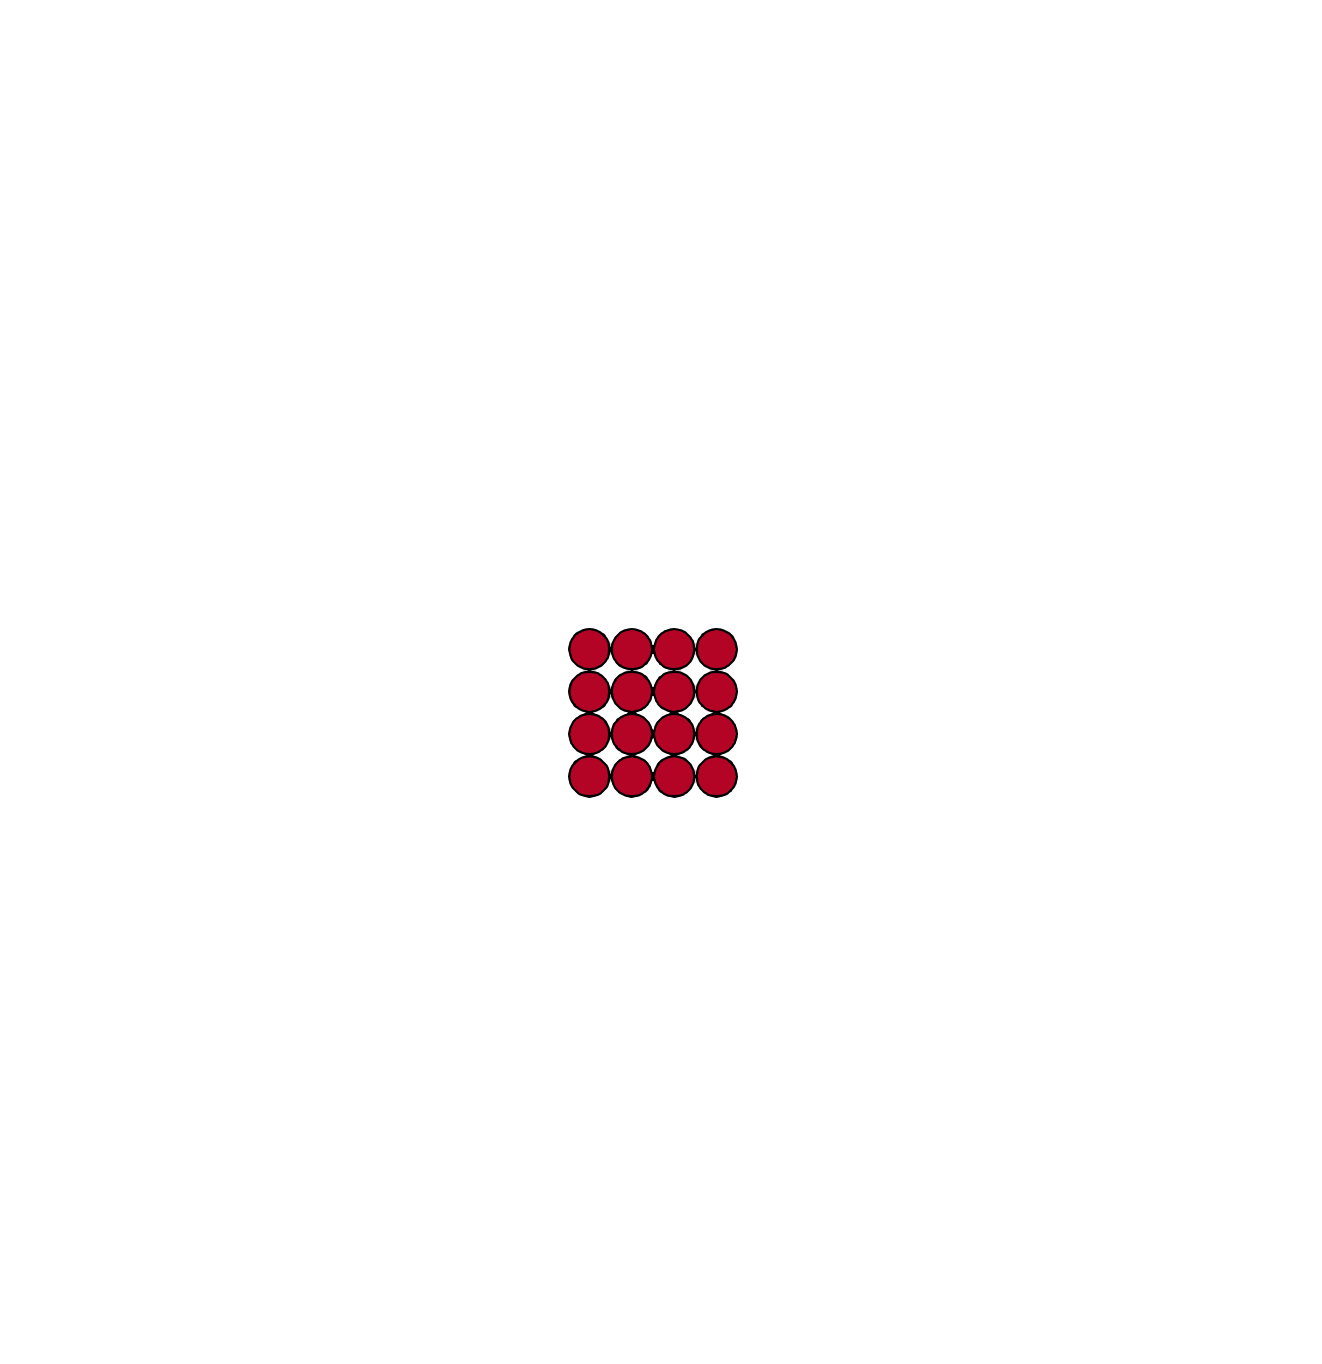
\includegraphics[width=0.95\linewidth]{../movies/NonCycling/image.0000.png}
    \caption{$t=0$ days}
  \end{subfigure}
  \hfill
  \begin{subfigure}[t]{0.31\textwidth}
    \centering
    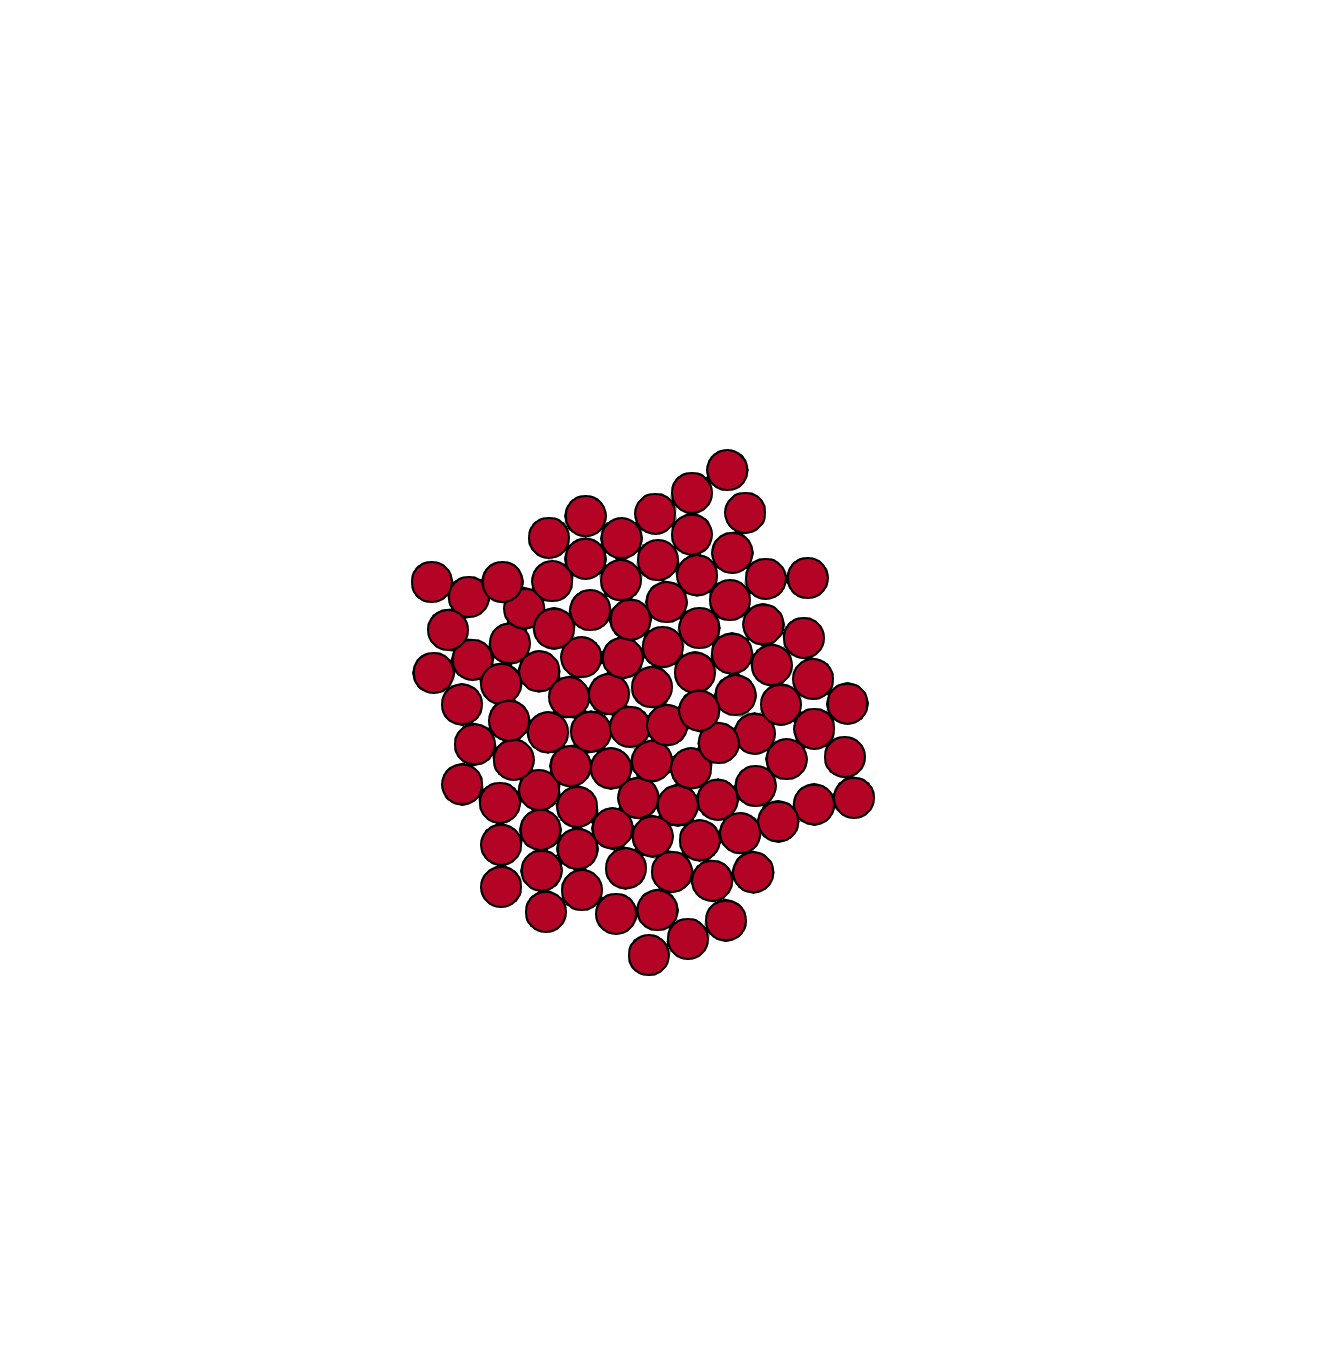
\includegraphics[width=0.95\linewidth]{../movies/NonCycling/image.0240.png}
    \caption{$t=5$ days}
  \end{subfigure}
  \hfill
  \begin{subfigure}[t]{0.31\textwidth}
    \centering
    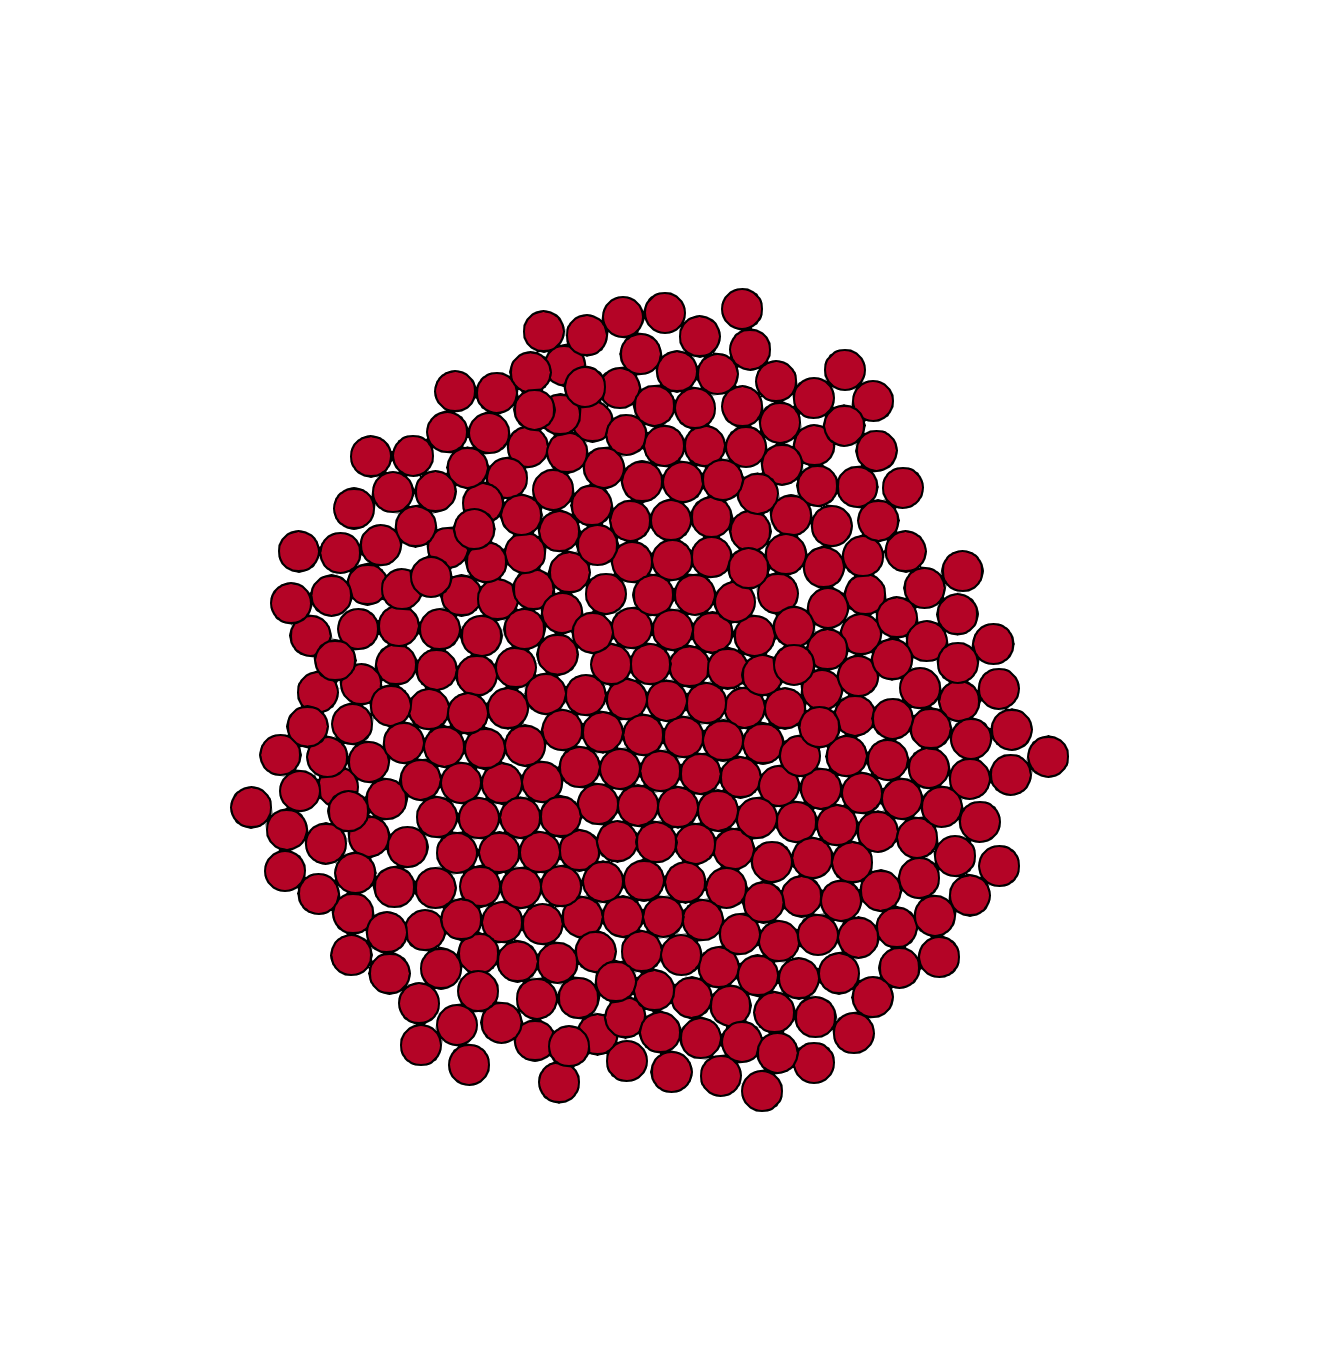
\includegraphics[width=0.95\linewidth]{../movies/NonCycling/image.0480.png}
    \caption{$t=10$ days}
  \end{subfigure}
  \\
  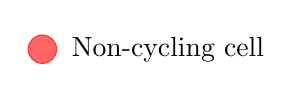
\begin{tikzpicture}
    \draw[fill=red!60,draw=red!80] (0,0) circle (0.18cm);
    \node[right] at (0.25,0) {Non-cycling cell};
  \end{tikzpicture}
  \\
  \begin{subfigure}[t]{0.72\textwidth}
    \centering
    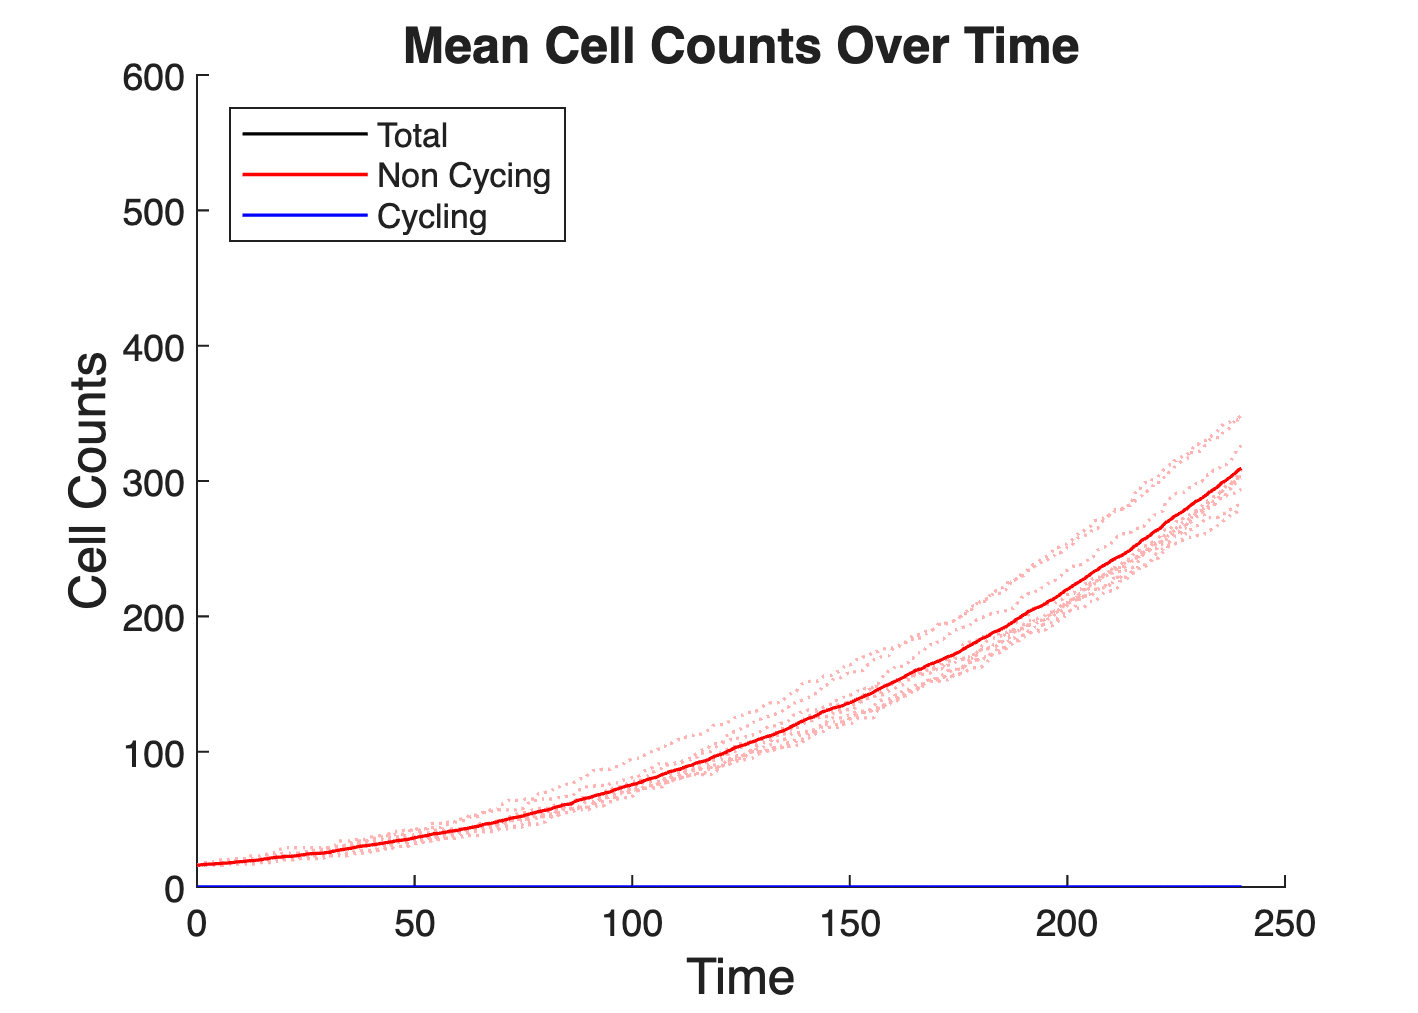
\includegraphics[width=0.95\linewidth]{../matlab/ClocksMonolayer_Cycling0_NonCycling16.png}
    \caption{Cell number over time}
  \end{subfigure}
  \caption{All Non-Cycling simulation group: snapshots and mean cell counts over time.}
  \label{fig:all-noncycling-results}
\end{figure}

\begin{figure}[htbp]
  \centering
  \begin{subfigure}[t]{0.31\textwidth}
    \centering
    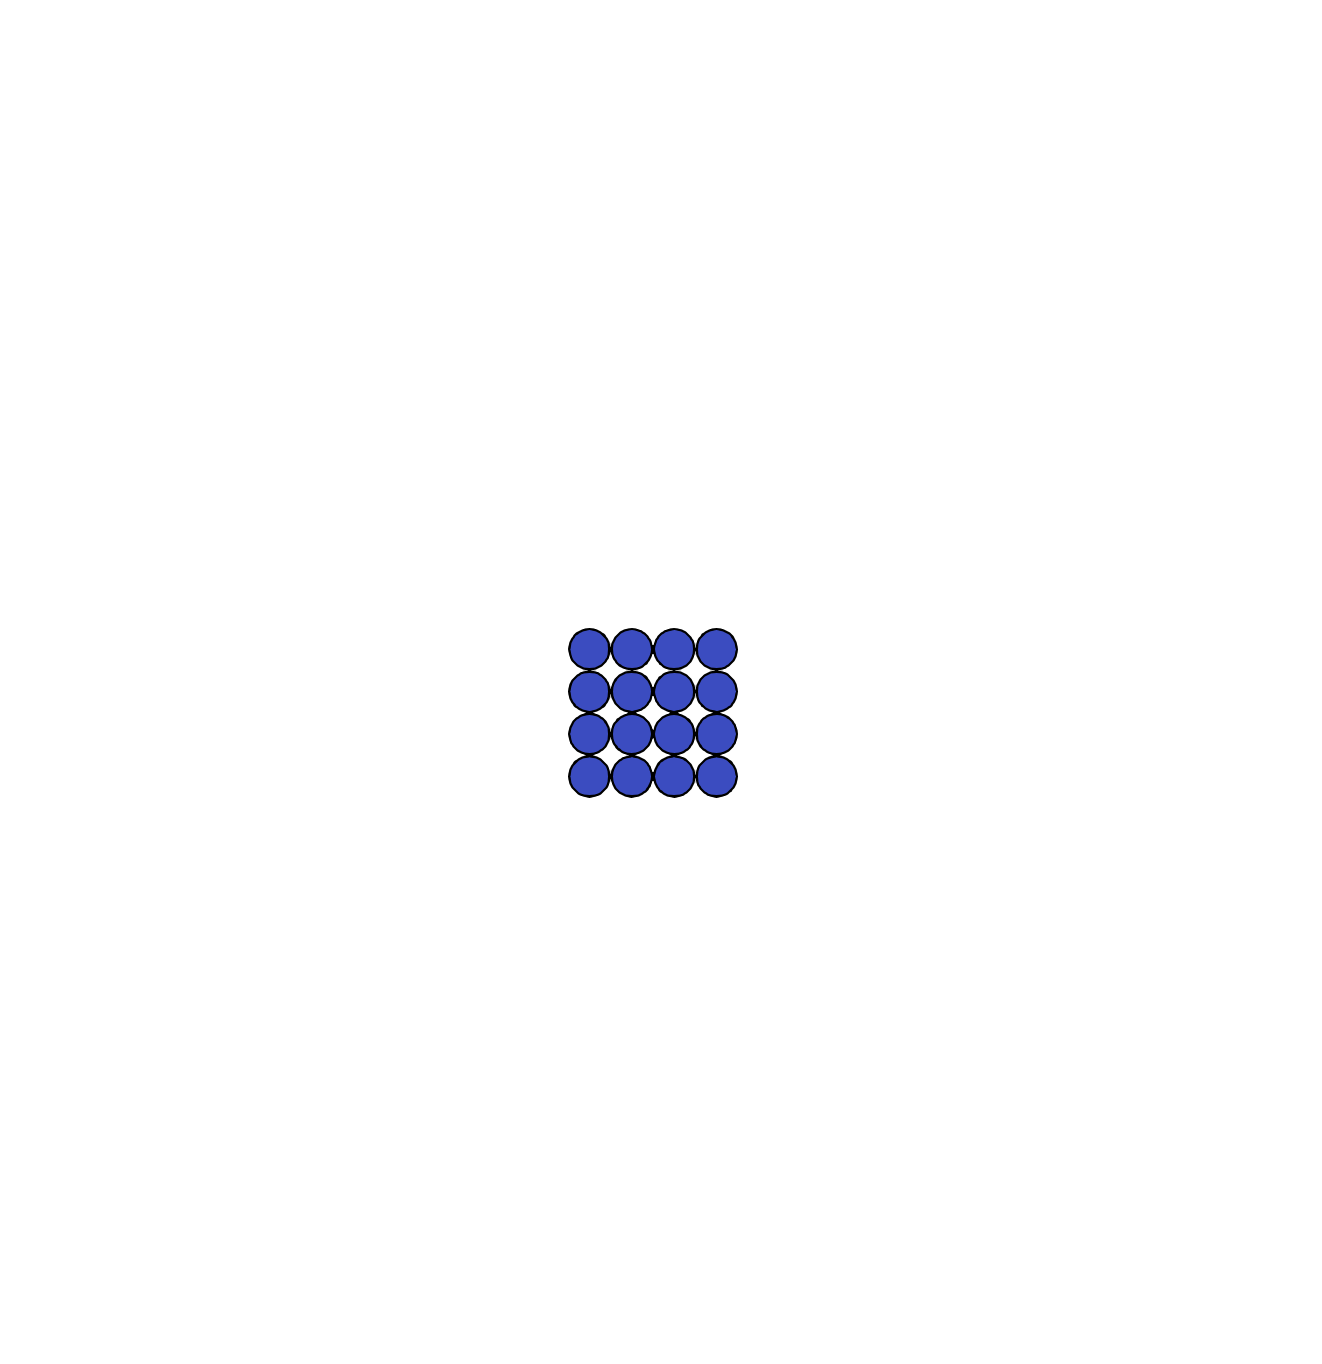
\includegraphics[width=0.95\linewidth]{../movies/Cycling/image.0000.png}
    \caption{$t=0$ days}
  \end{subfigure}
  \hfill
  \begin{subfigure}[t]{0.31\textwidth}
    \centering
    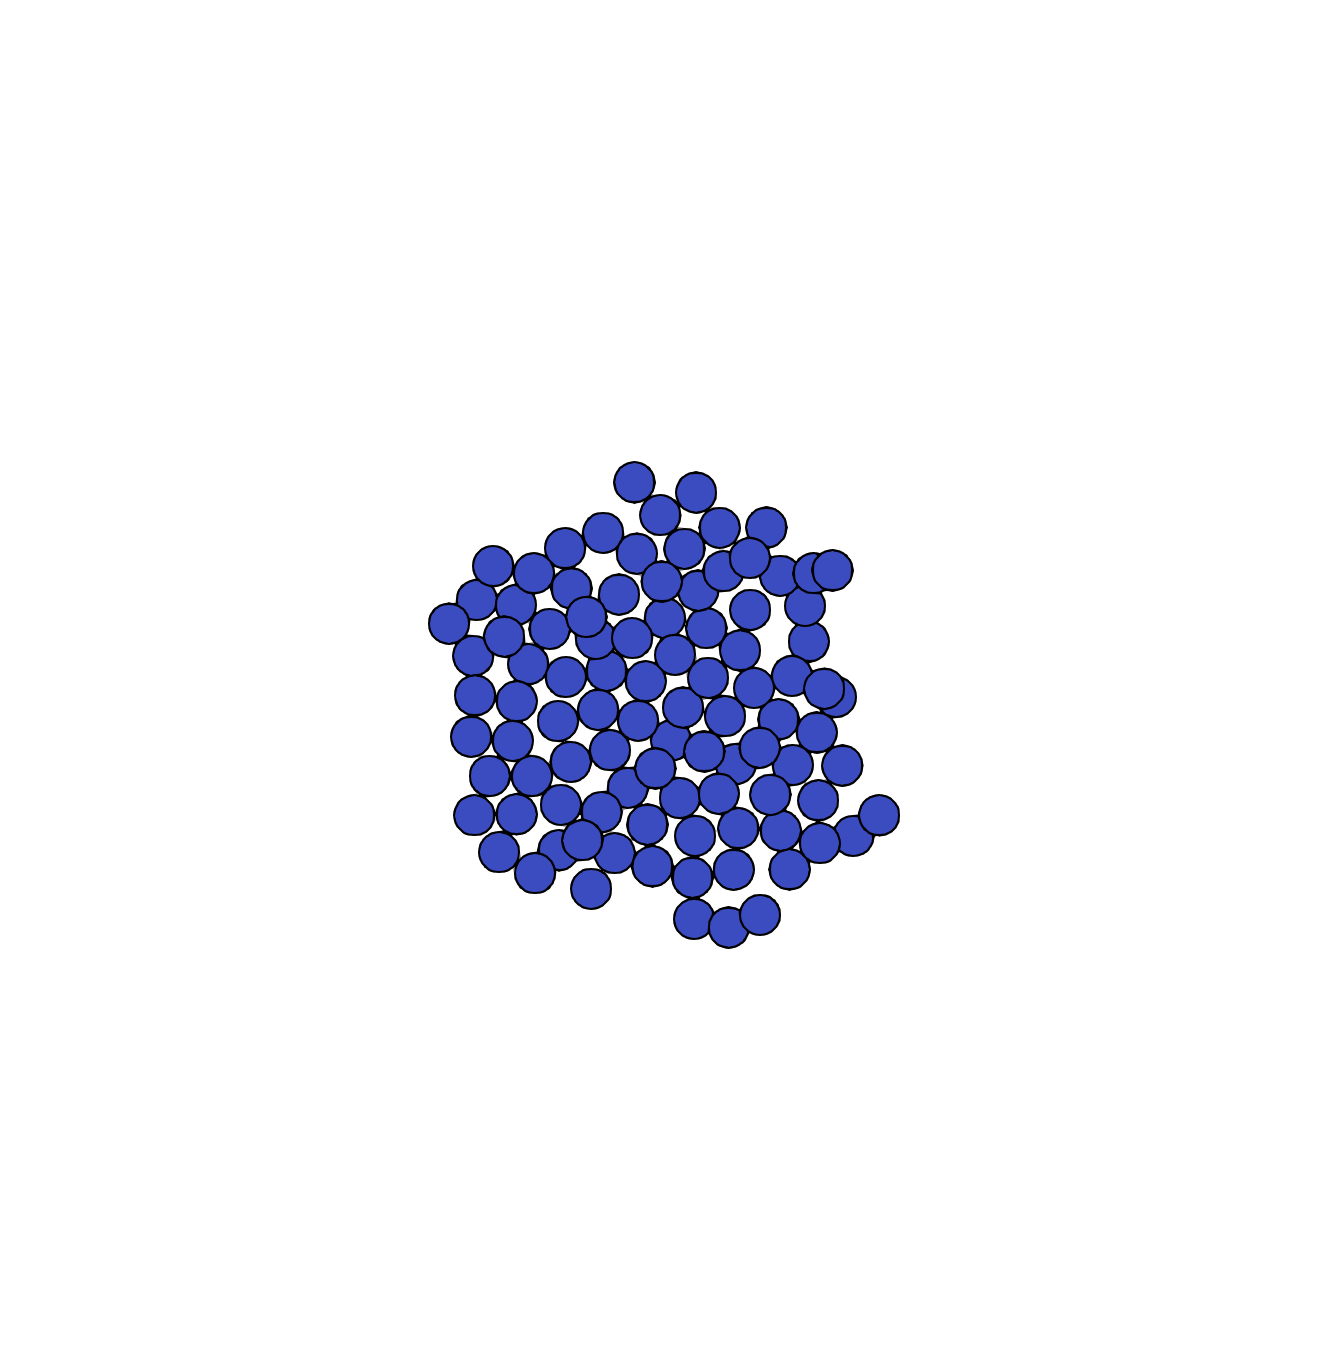
\includegraphics[width=0.95\linewidth]{../movies/Cycling/image.0240.png}
    \caption{$t=5$ days}
  \end{subfigure}
  \hfill
  \begin{subfigure}[t]{0.31\textwidth}
    \centering
    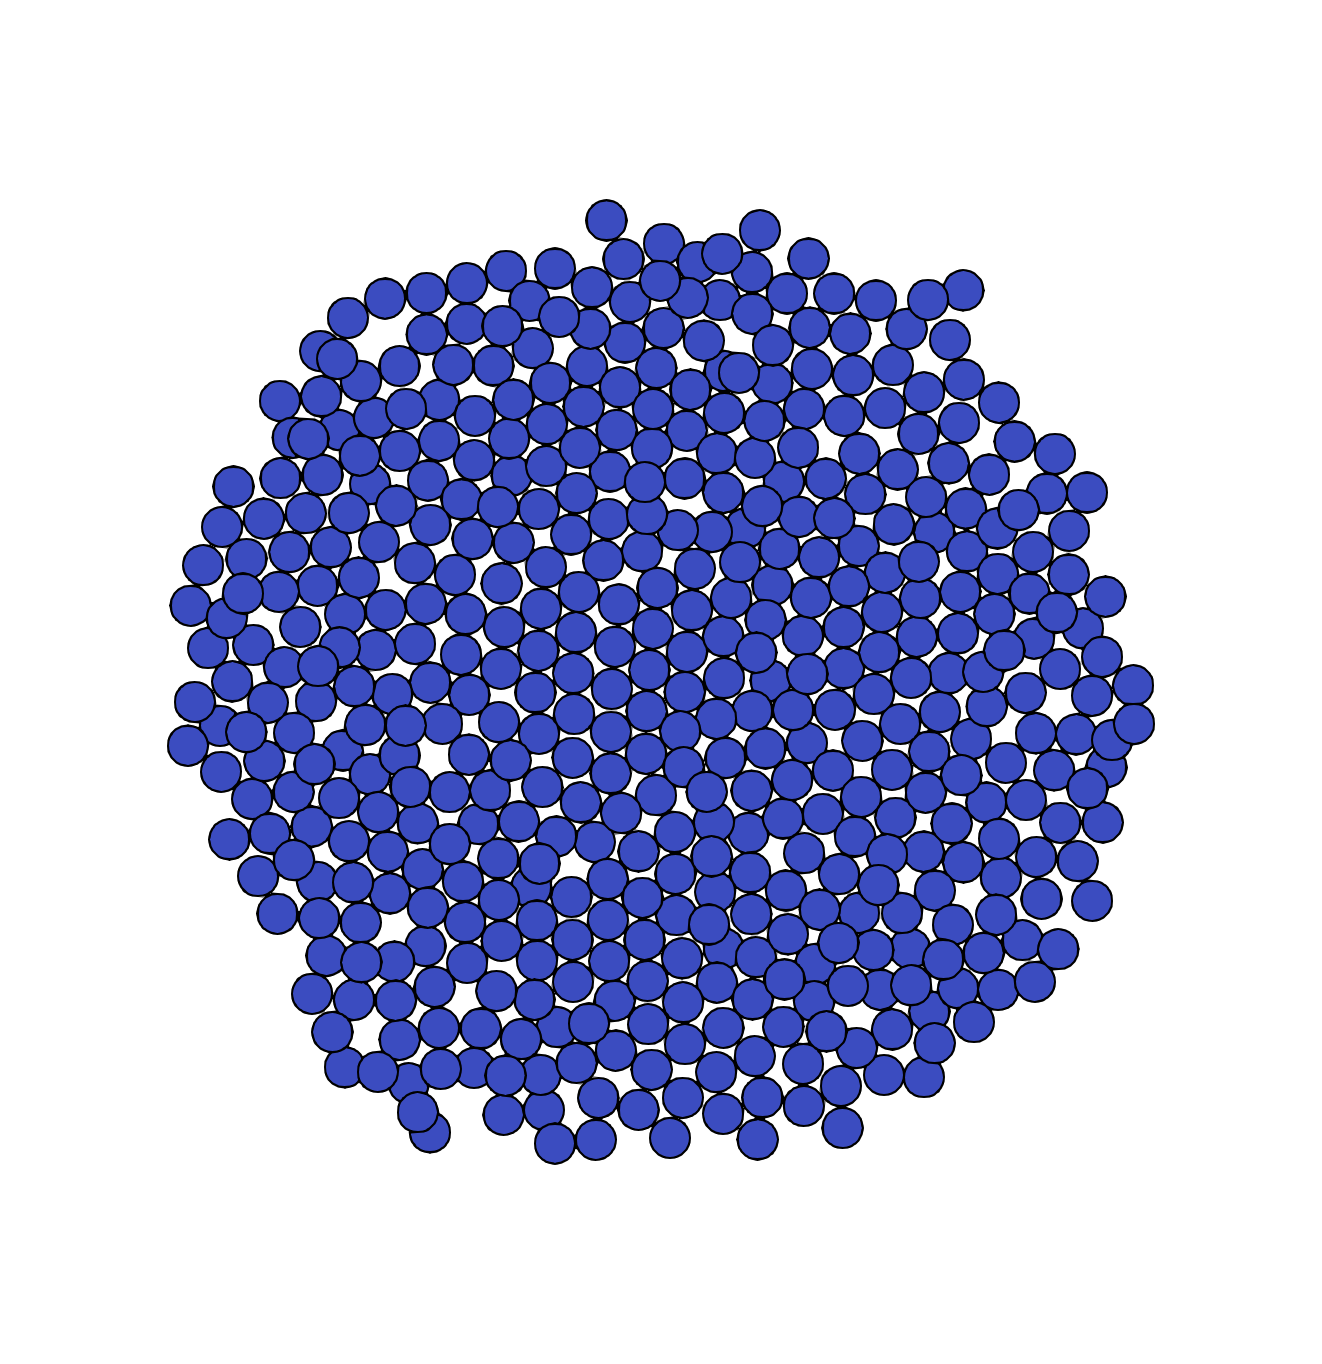
\includegraphics[width=0.95\linewidth]{../movies/Cycling/image.0480.png}
    \caption{$t=10$ days}
  \end{subfigure}
  \\
   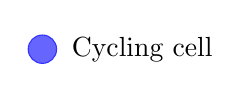
\begin{tikzpicture}
    \draw[fill=blue!60,draw=blue!80] (0,0) circle (0.18cm);
    \node[right] at (0.25,0) {Cycling cell};
  \end{tikzpicture}
  \\
  \begin{subfigure}[t]{0.72\textwidth}
    \centering
    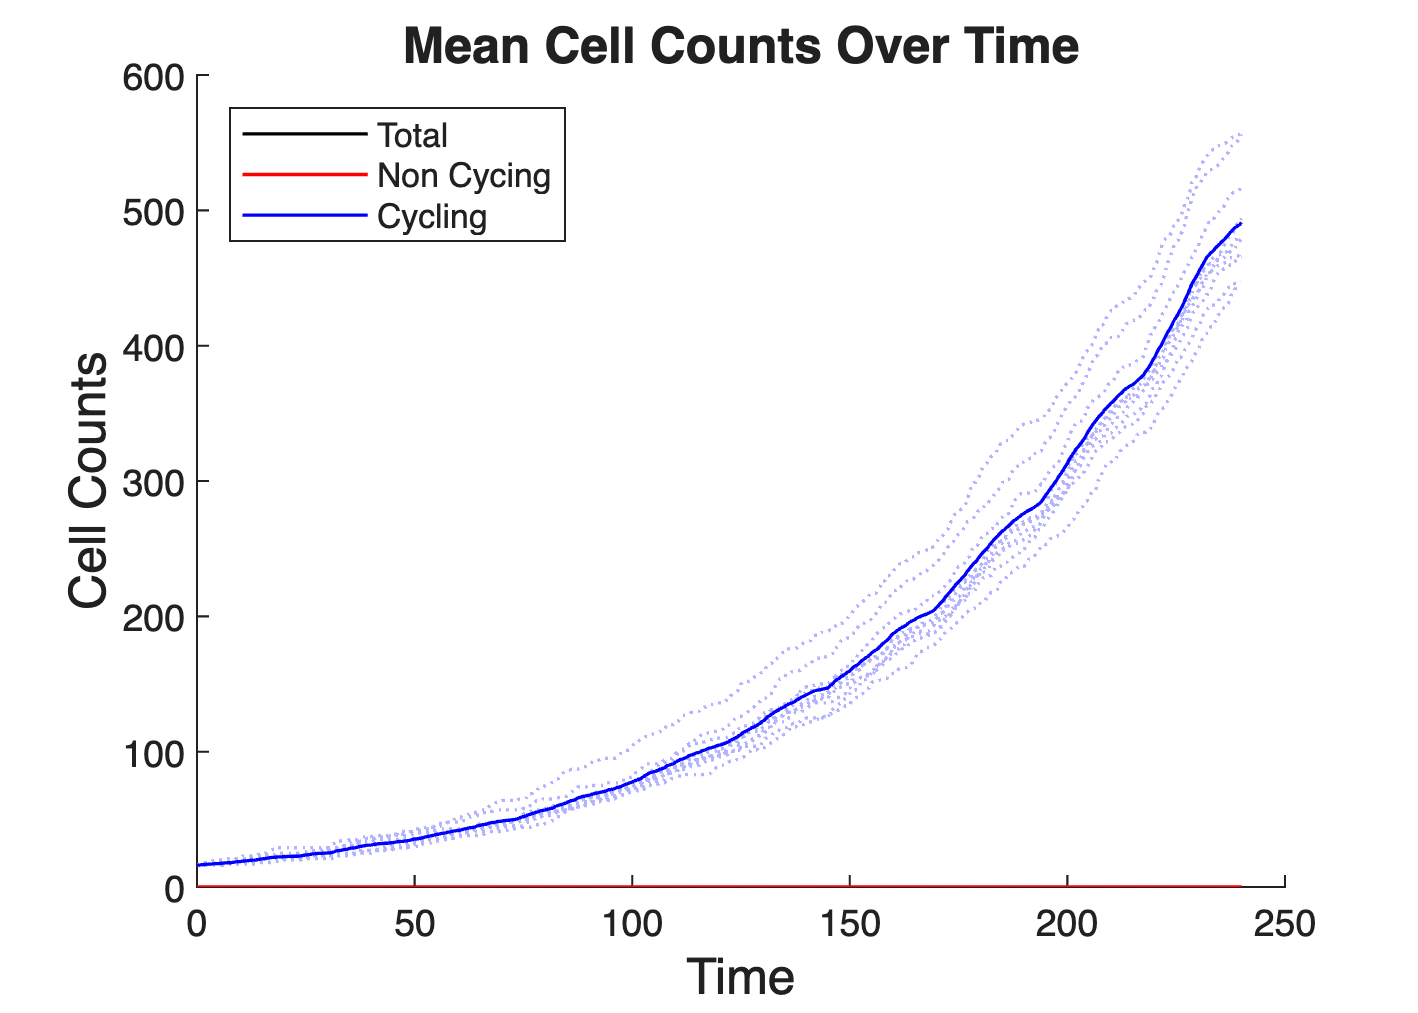
\includegraphics[width=0.95\linewidth]{../matlab/ClocksMonolayer_Cycling16_NonCycling0.png}
    \caption{Cell number over time}
  \end{subfigure}
  \caption{All Cycling simulation group: snapshots and mean cell counts over time. Cell colour indicates drag phase.}
  \label{fig:all-cycling-results}
\end{figure}

\begin{figure}[htbp]
  \centering
  \begin{subfigure}[t]{0.31\textwidth}
    \centering
    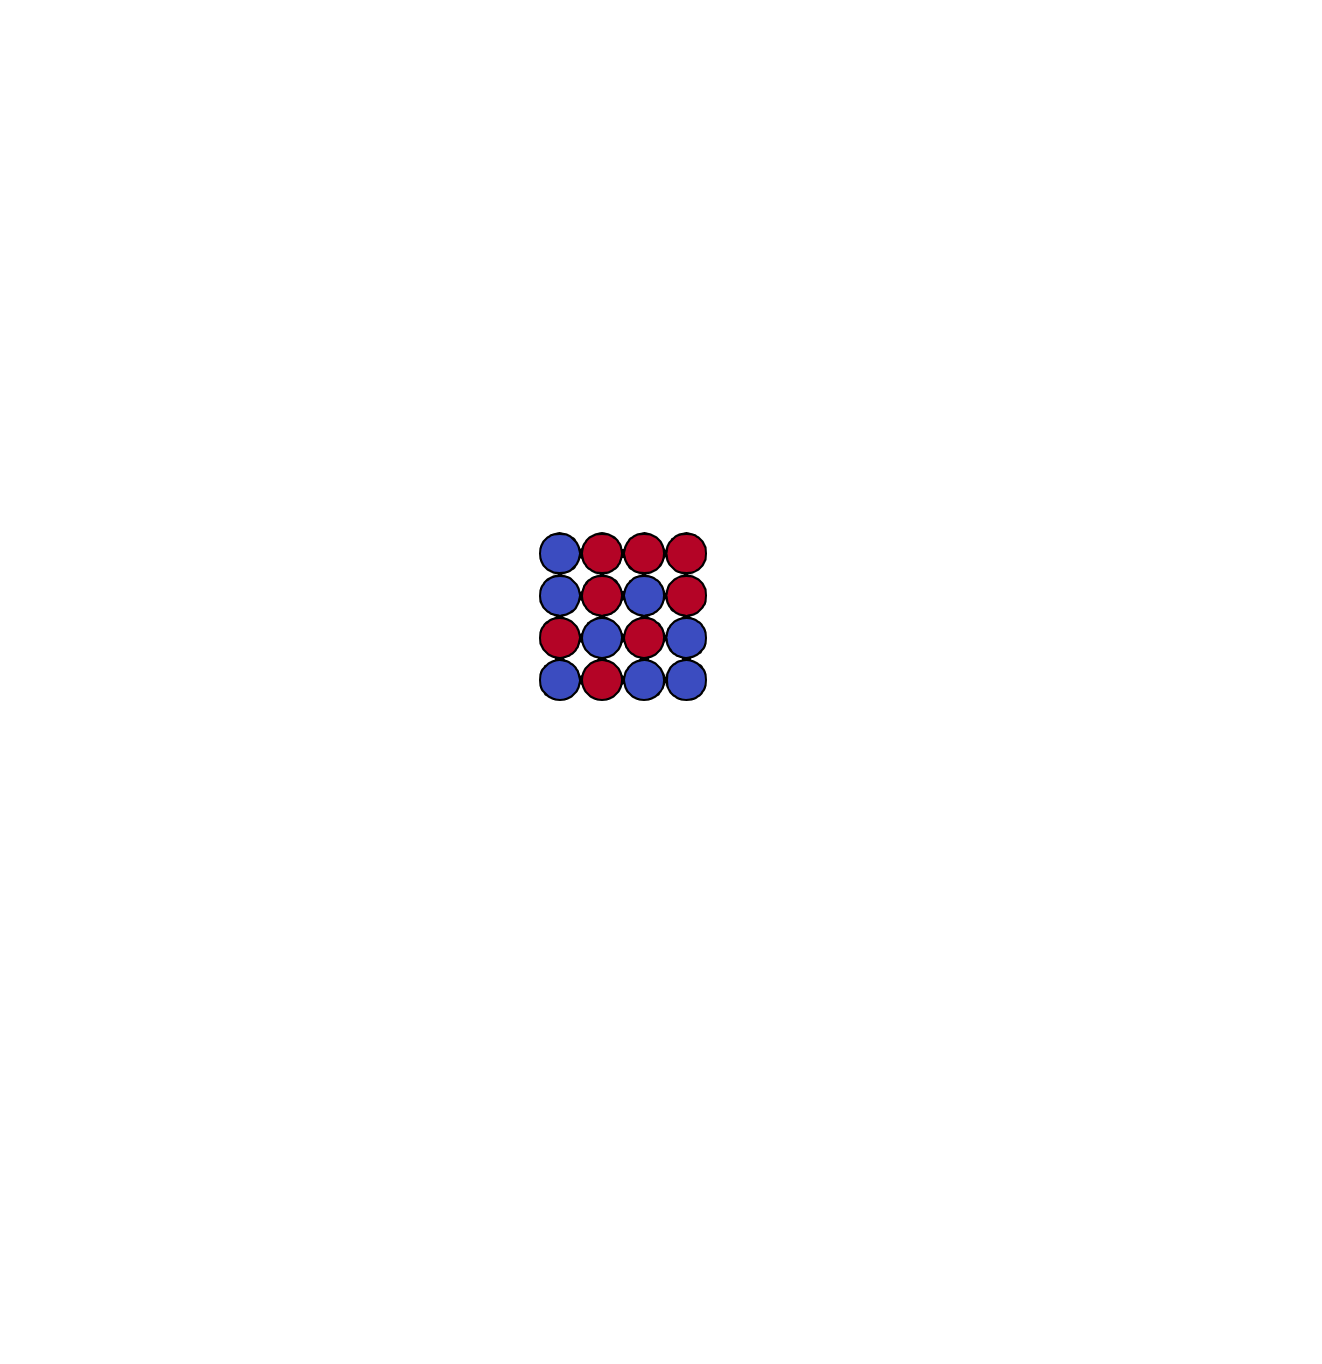
\includegraphics[width=0.95\linewidth]{../movies/Mixed/image.0000.png}
    \caption{$t=0$ days}
  \end{subfigure}
  \hfill
  \begin{subfigure}[t]{0.31\textwidth}
    \centering
    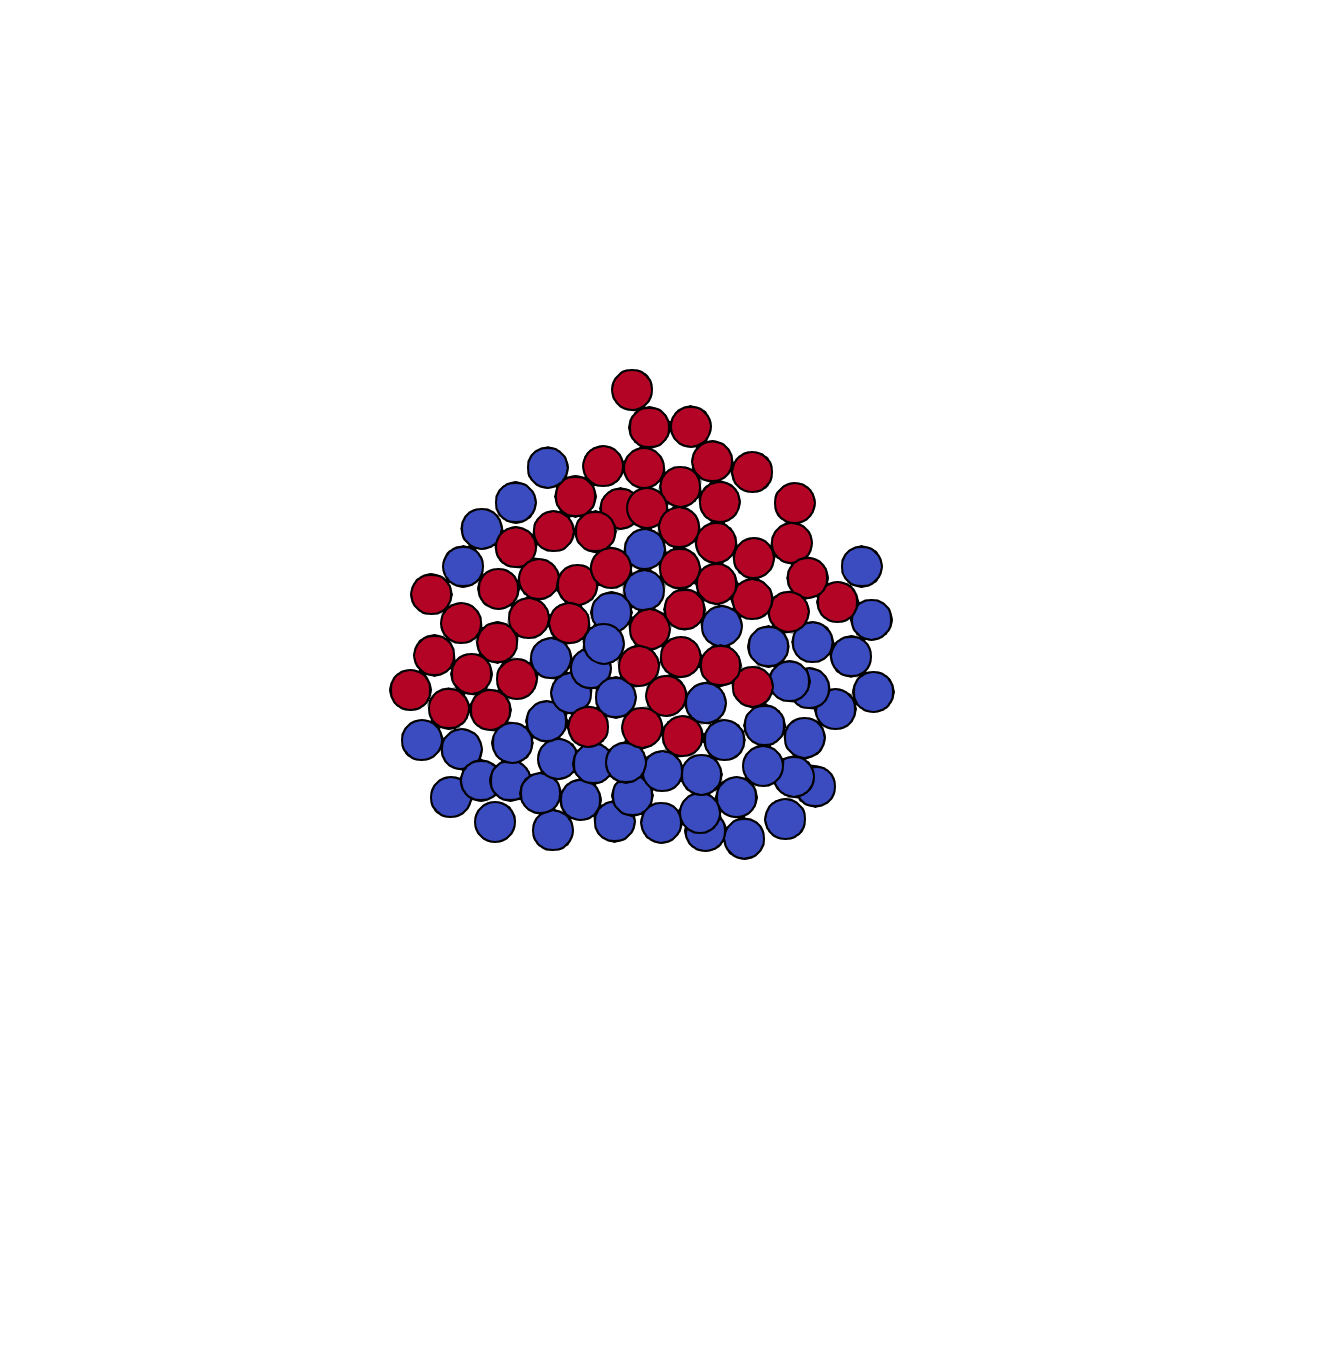
\includegraphics[width=0.95\linewidth]{../movies/Mixed/image.0240.png}
    \caption{$t=5$ days}
  \end{subfigure}
  \hfill
  \begin{subfigure}[t]{0.31\textwidth}
    \centering
    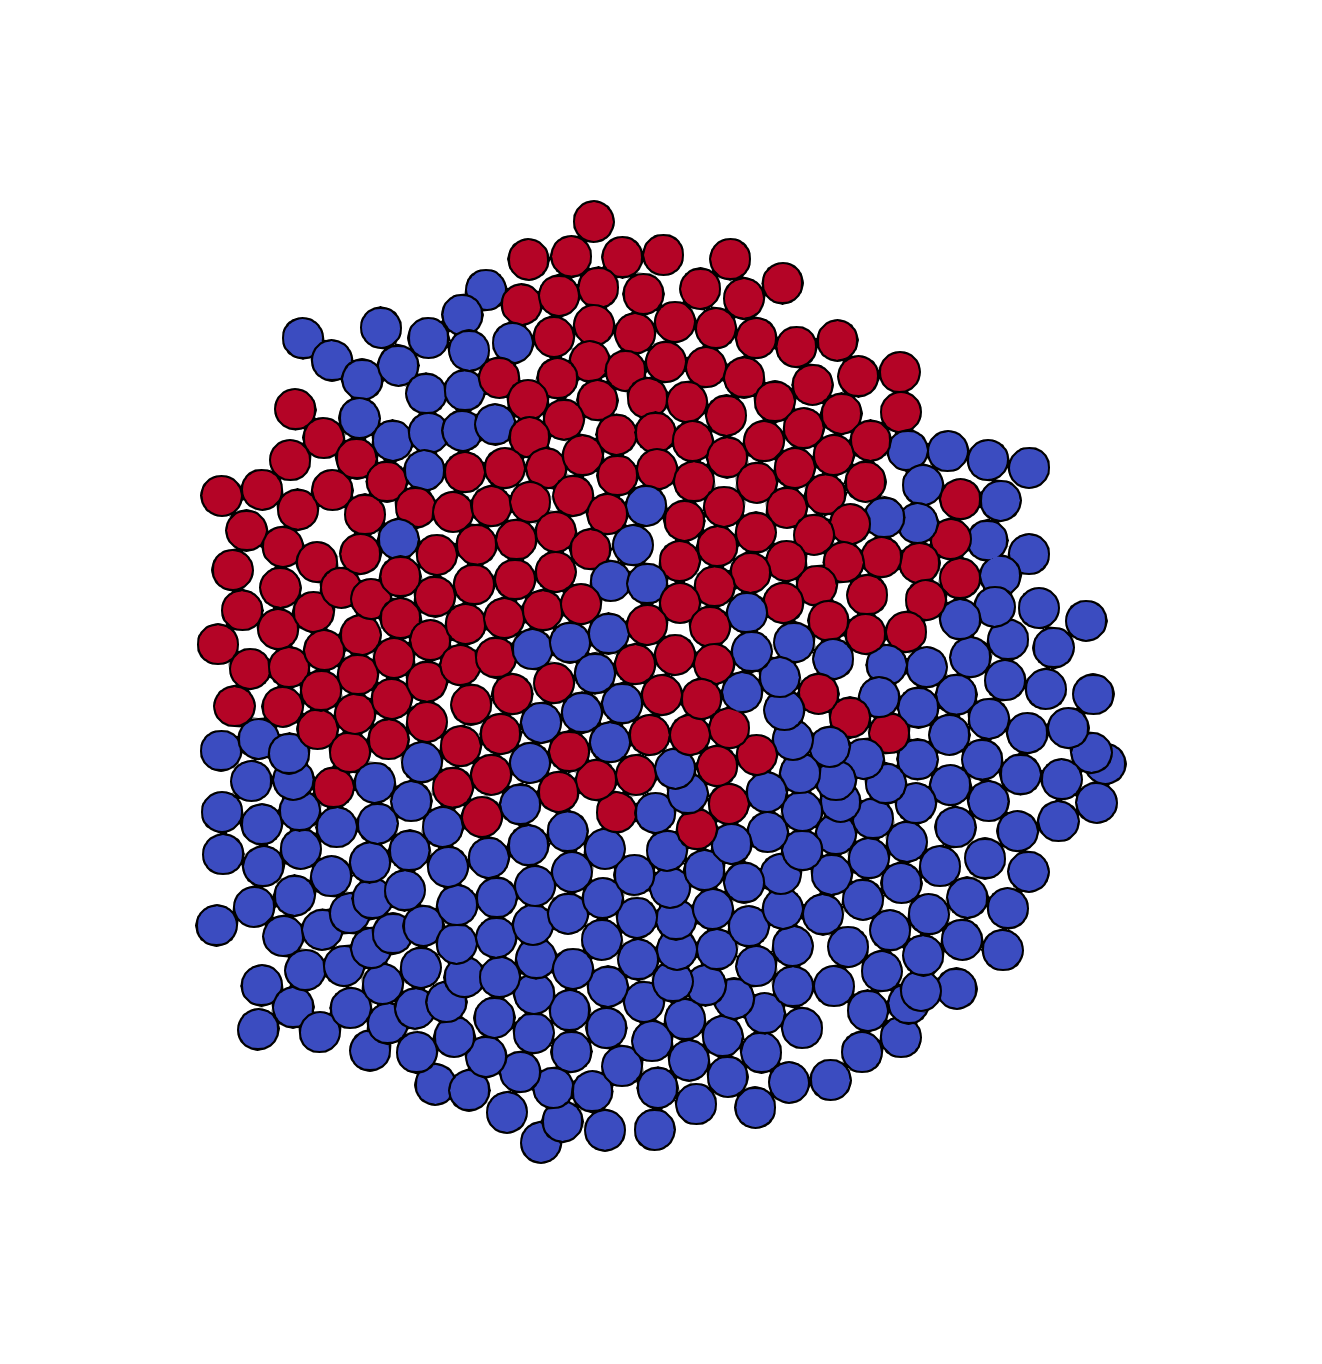
\includegraphics[width=0.95\linewidth]{../movies/Mixed/image.0480.png}
    \caption{$t=10$ days}
  \end{subfigure}
  \\
  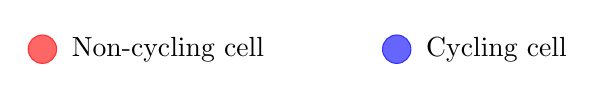
\begin{tikzpicture}
    \draw[fill=red!60,draw=red!80] (0,0) circle (0.18cm);
    \node[right] at (0.25,0) {Non-cycling cell};
    \draw[fill=blue!60,draw=blue!80] (4.5,0) circle (0.18cm);
    \node[right] at (4.75,0) {Cycling cell};
  \end{tikzpicture}
  \\
  \begin{subfigure}[t]{0.72\textwidth}
    \centering
    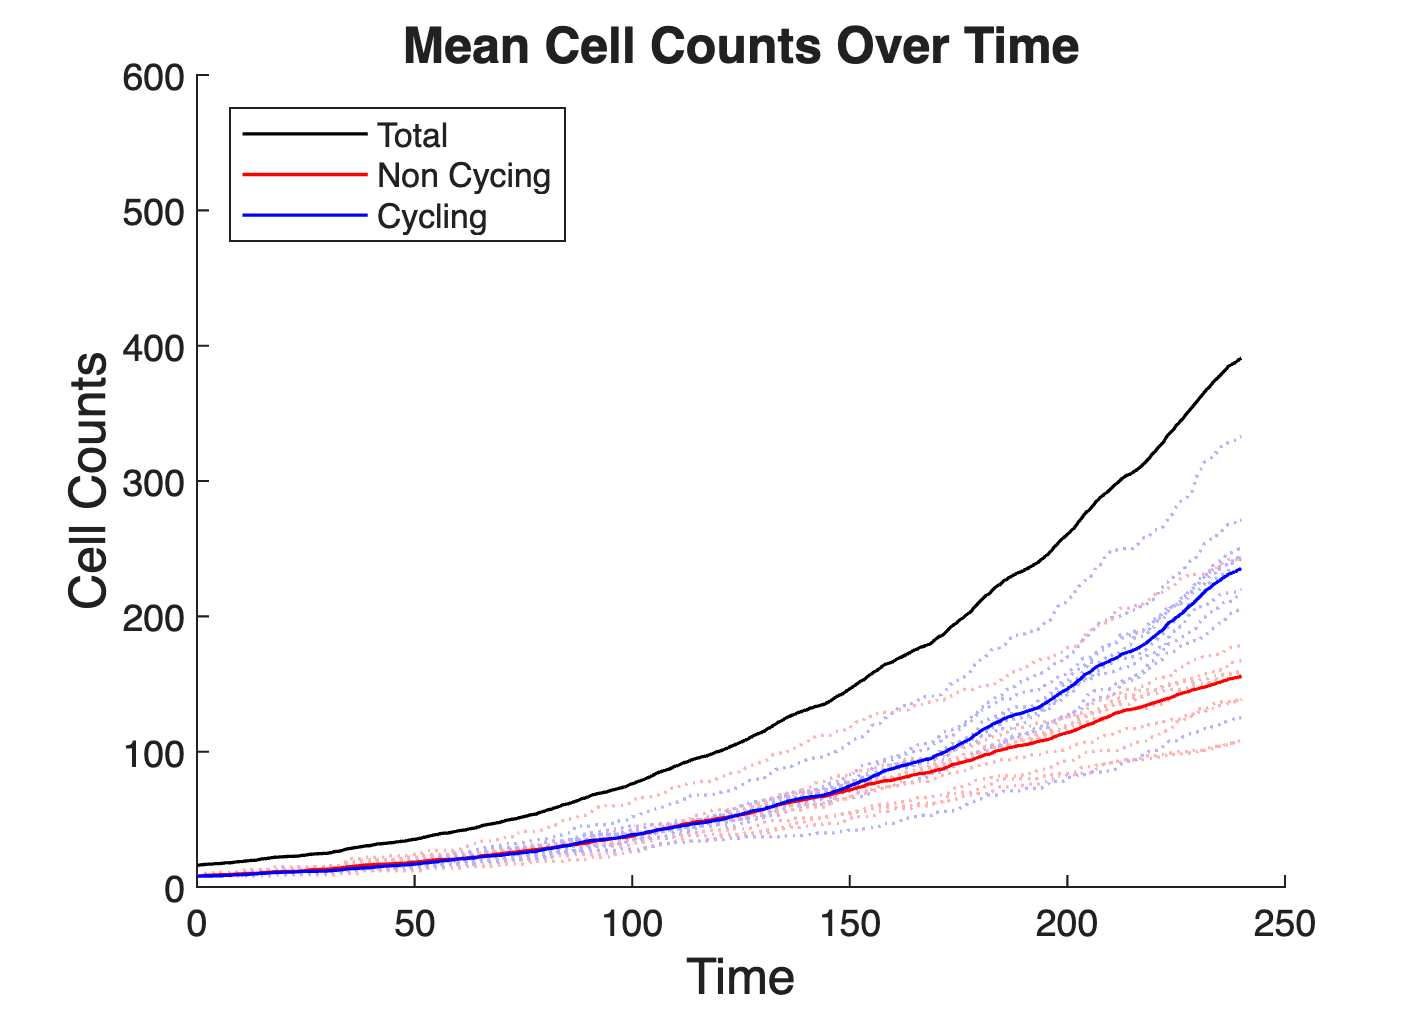
\includegraphics[width=0.95\linewidth]{../matlab/ClocksMonolayer_Cycling8_NonCycling8.png}
    \caption{Cell number over time}
  \end{subfigure}
  \caption{Half Non-Cycling / Half Cycling simulation group: snapshots and mean cell counts over time. Cell colour indicates phenotype and drag phase.}
  \label{fig:half-half-results}
\end{figure}

These results support the model interpretation that periodic drag modulation in
cycling cells alters collective dynamics compared with constant-drag non-cycling
cells, and that mixed populations interpolate between homogeneous limits.

\begin{figure}[p]
  \raggedright%
  \begin{minipage}[c]{0.88\textwidth}
    \begin{subfigure}[t]{0.19\textwidth}
      \centering
      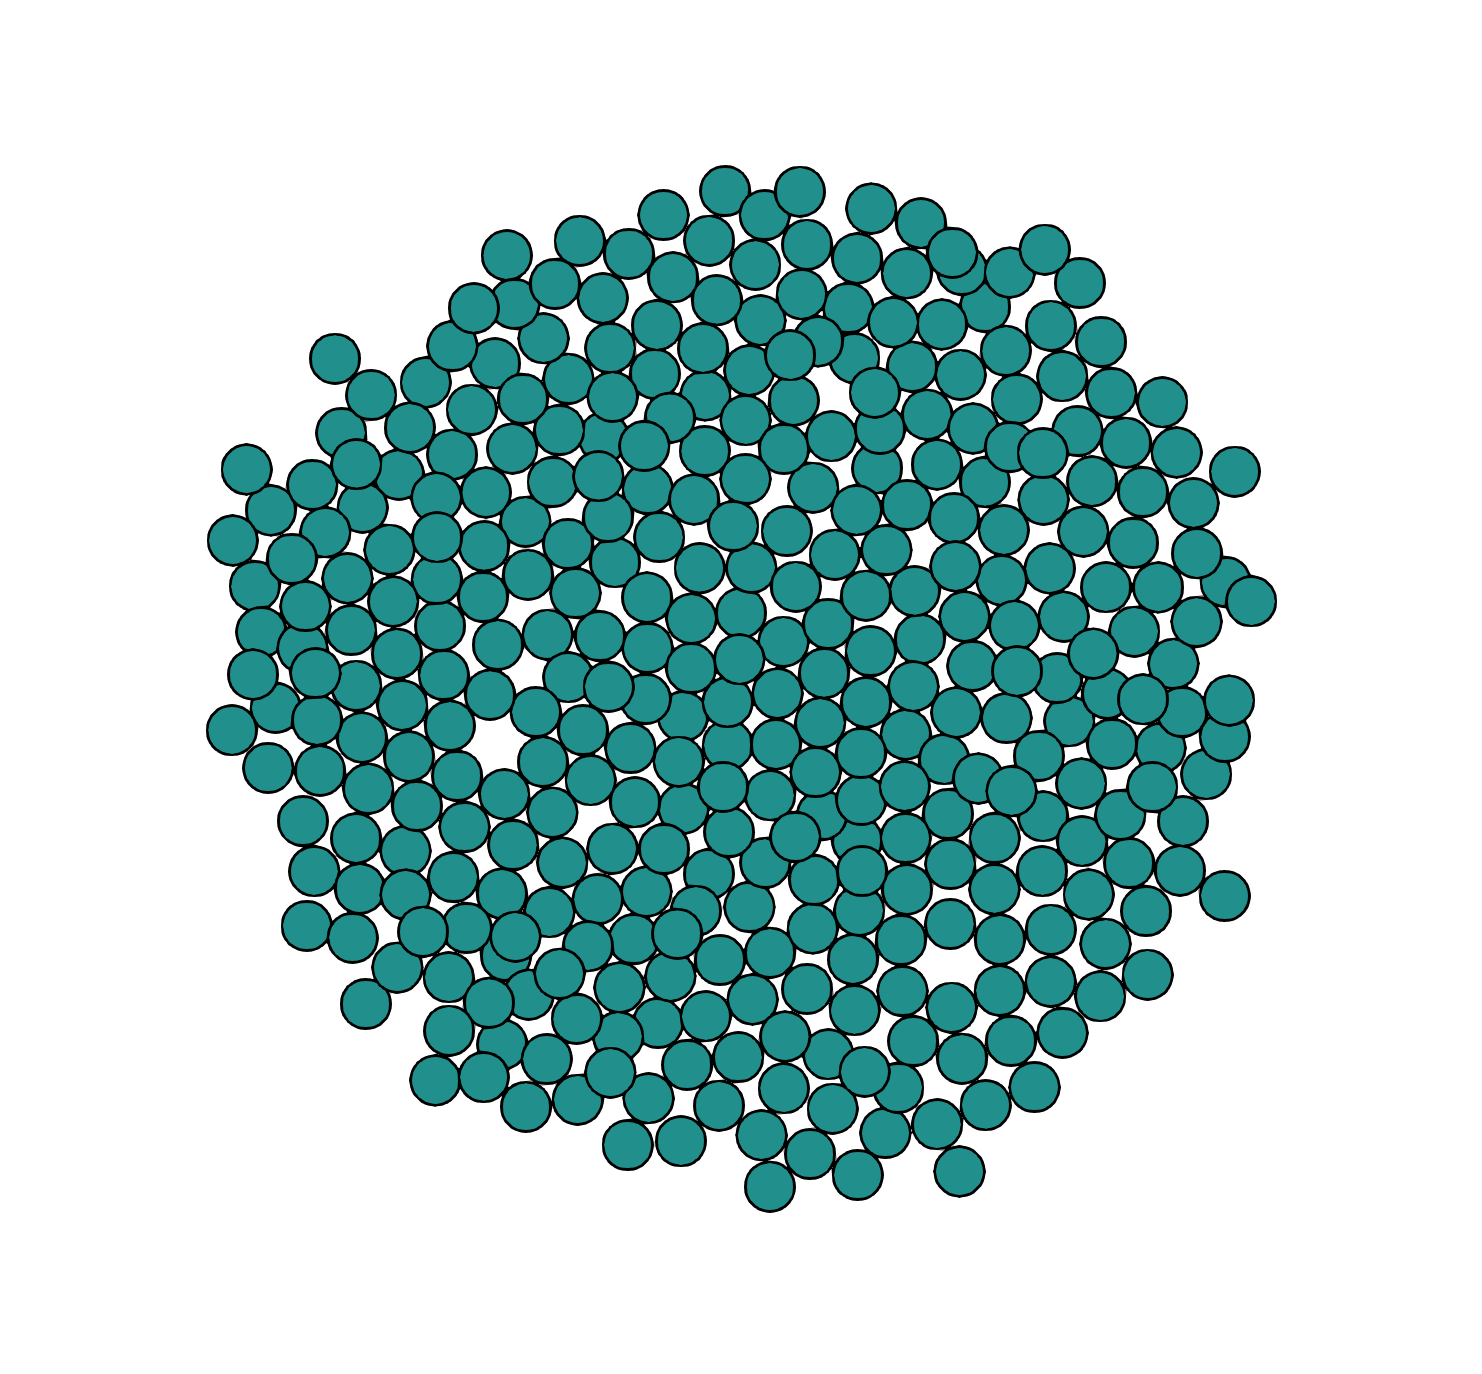
\includegraphics[width=\linewidth,trim=100 80 100 80,clip]{../movies/CyclingClock/image.0432.png}
      \caption{$t=0$ h}
    \end{subfigure}
    \hfill
    \begin{subfigure}[t]{0.19\textwidth}
      \centering
      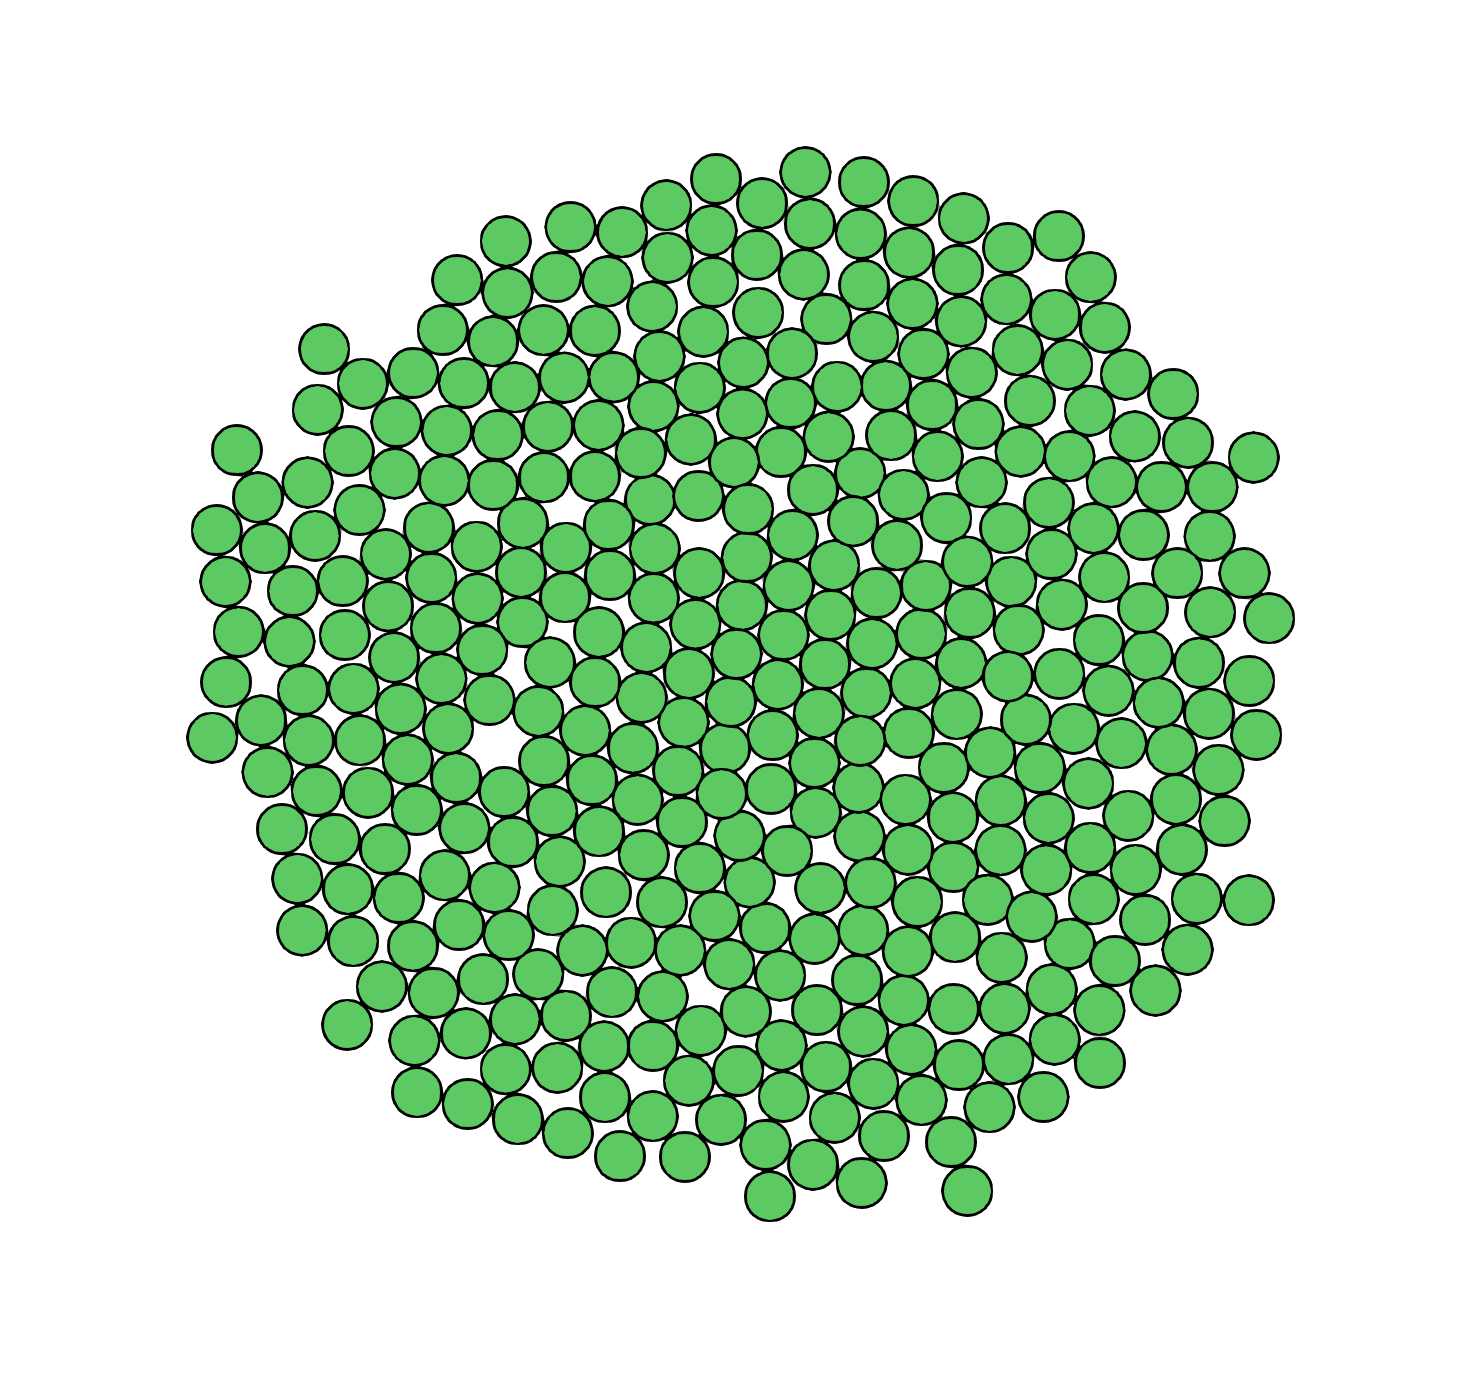
\includegraphics[width=\linewidth,trim=100 80 100 80,clip]{../movies/CyclingClock/image.0436.png}
      \caption{$t=2$ h}
    \end{subfigure}
    \hfill
    \begin{subfigure}[t]{0.19\textwidth}
      \centering
      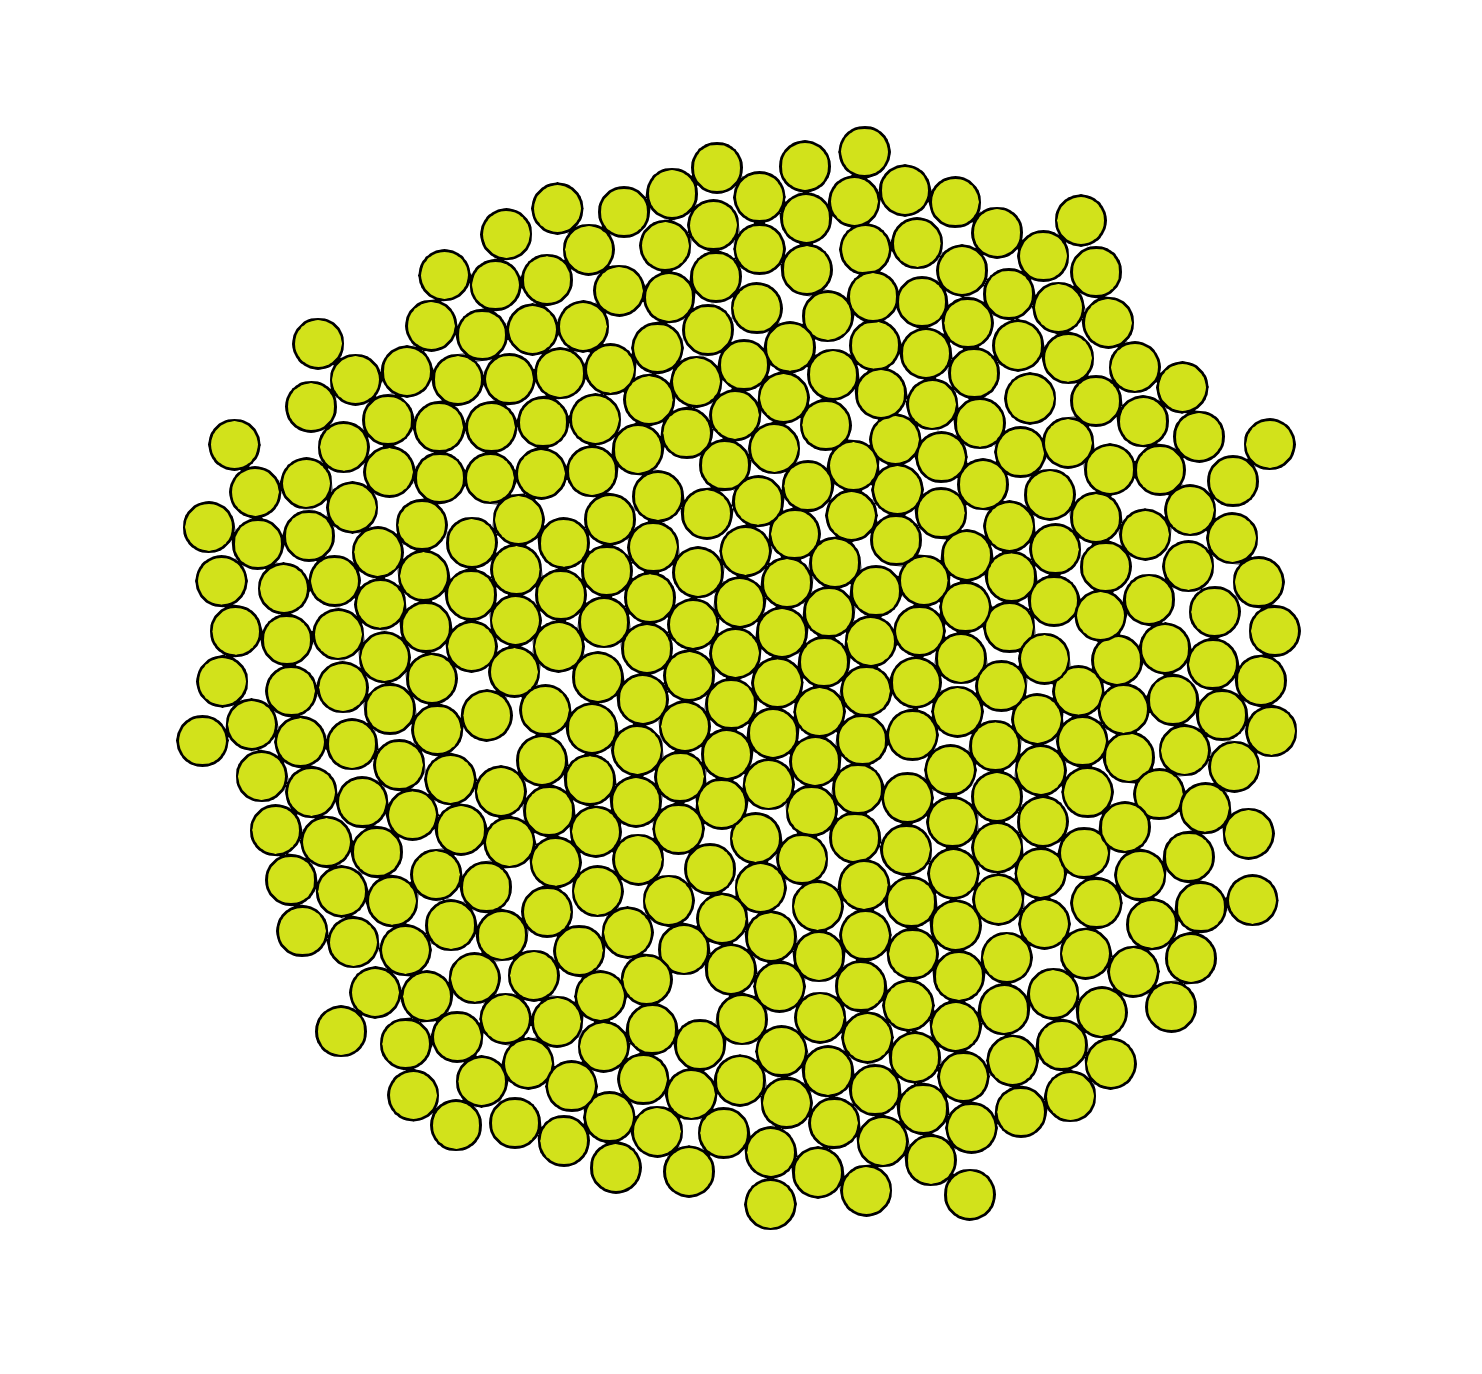
\includegraphics[width=\linewidth,trim=100 80 100 80,clip]{../movies/CyclingClock/image.0440.png}
      \caption{$t=4$ h}
    \end{subfigure}
    \hfill
    \begin{subfigure}[t]{0.19\textwidth}
      \centering
      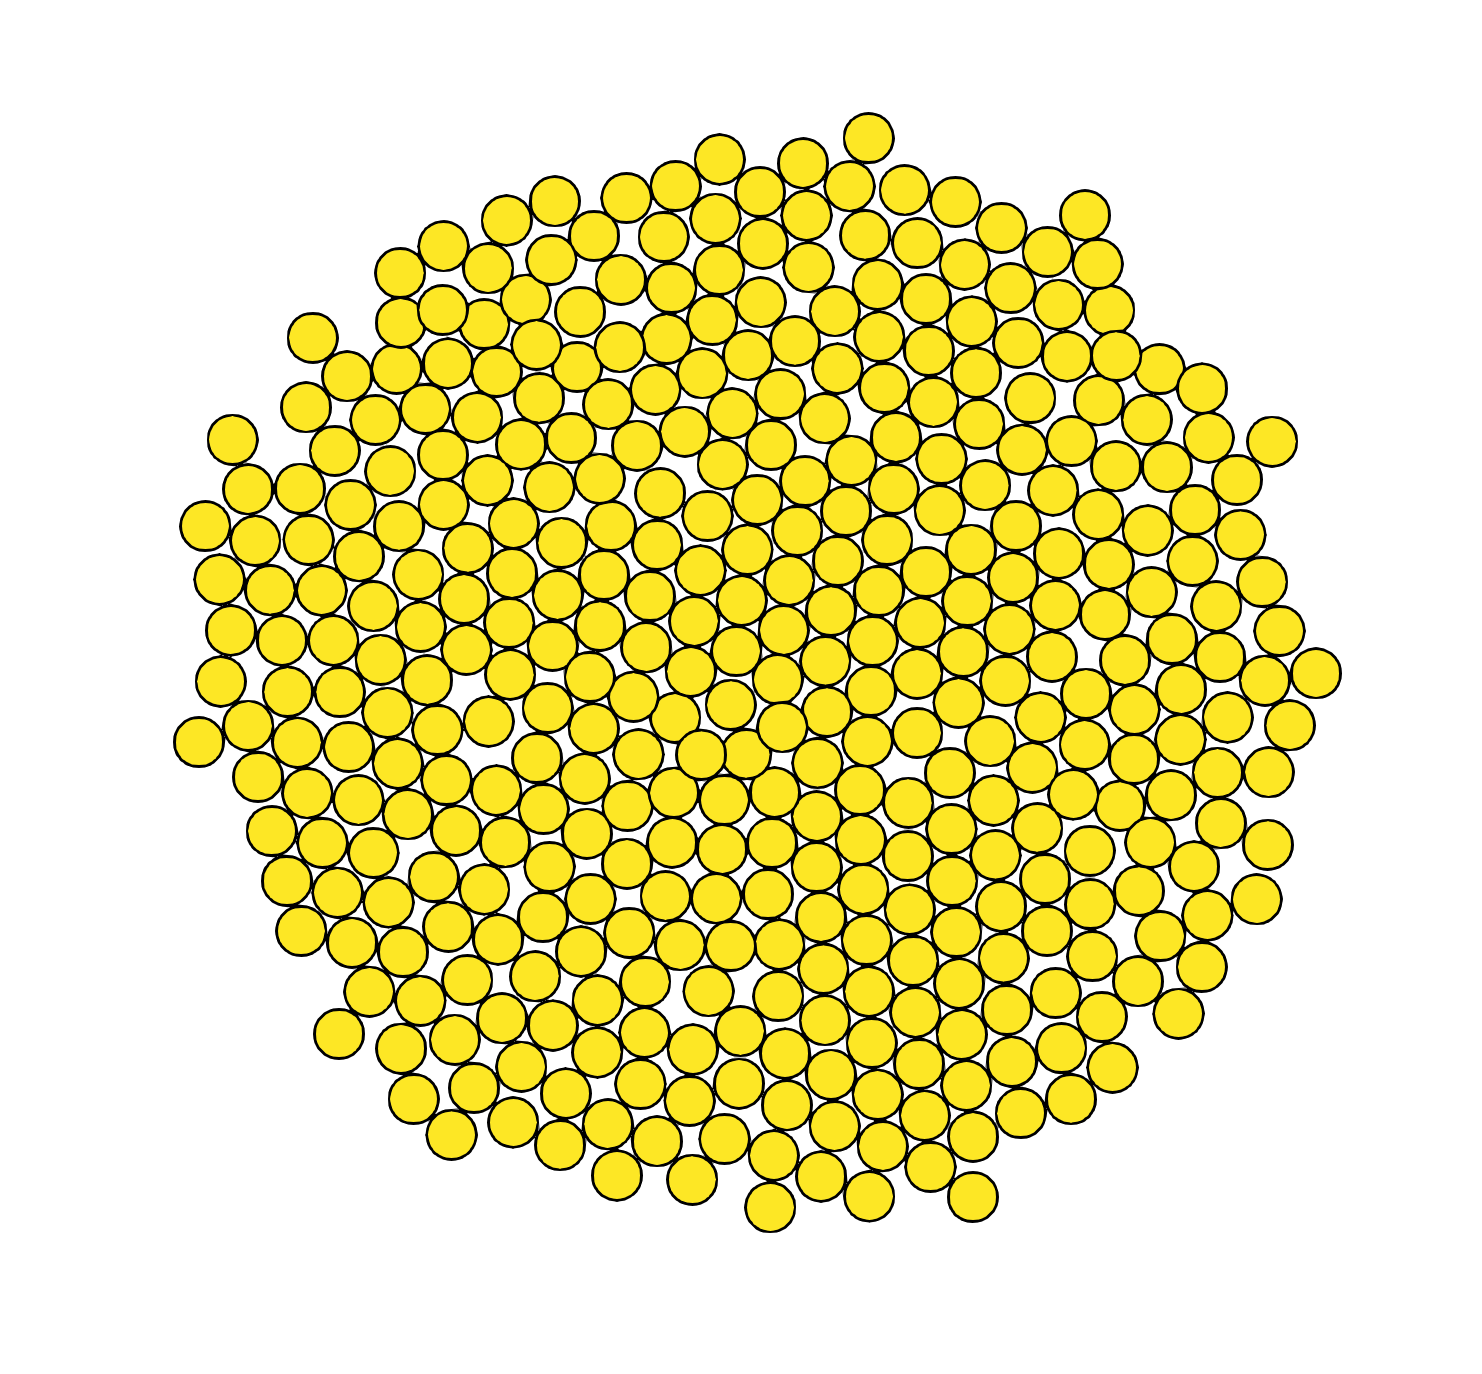
\includegraphics[width=\linewidth,trim=100 80 100 80,clip]{../movies/CyclingClock/image.0444.png}
      \caption{$t=6$ h}
    \end{subfigure}
    \hfill
    \begin{subfigure}[t]{0.19\textwidth}
      \centering
      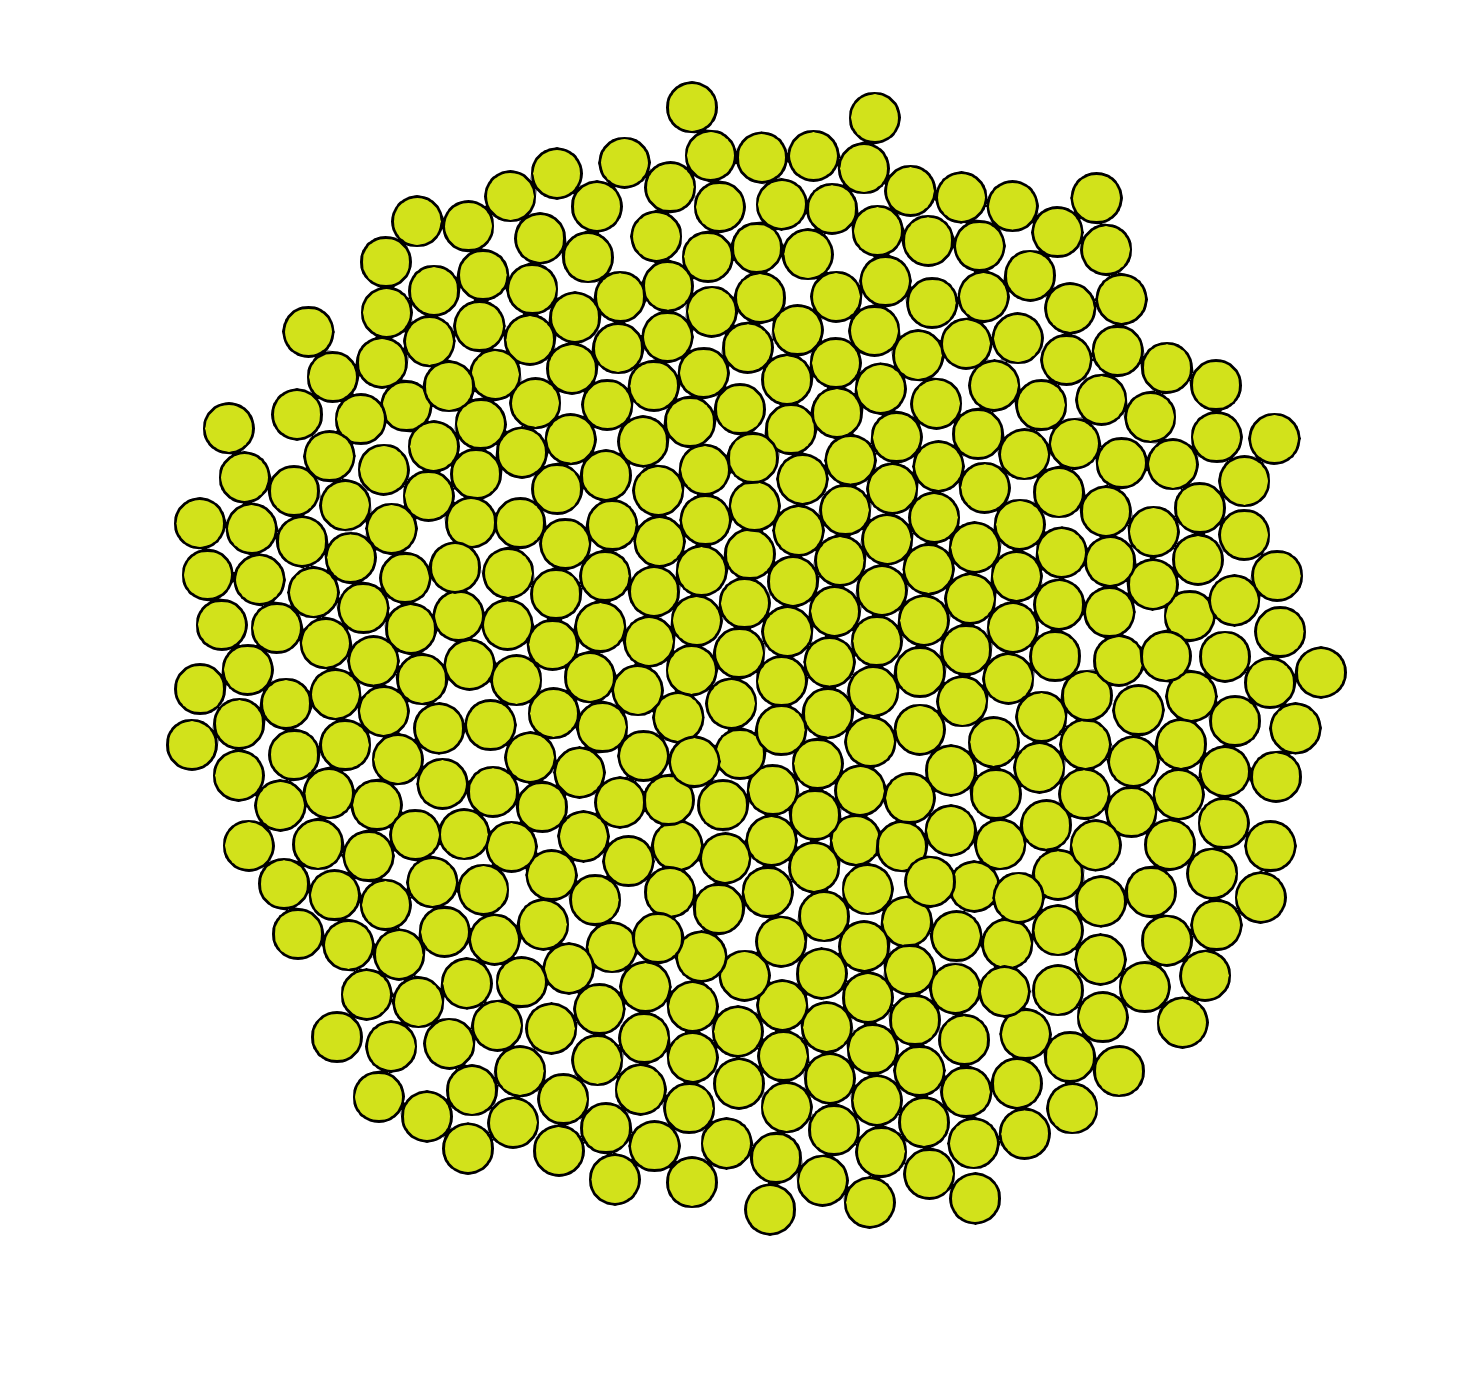
\includegraphics[width=\linewidth,trim=100 80 100 80,clip]{../movies/CyclingClock/image.0448.png}
      \caption{$t=8$ h}
    \end{subfigure}

    \medskip
    \begin{subfigure}[t]{0.19\textwidth}
      \centering
      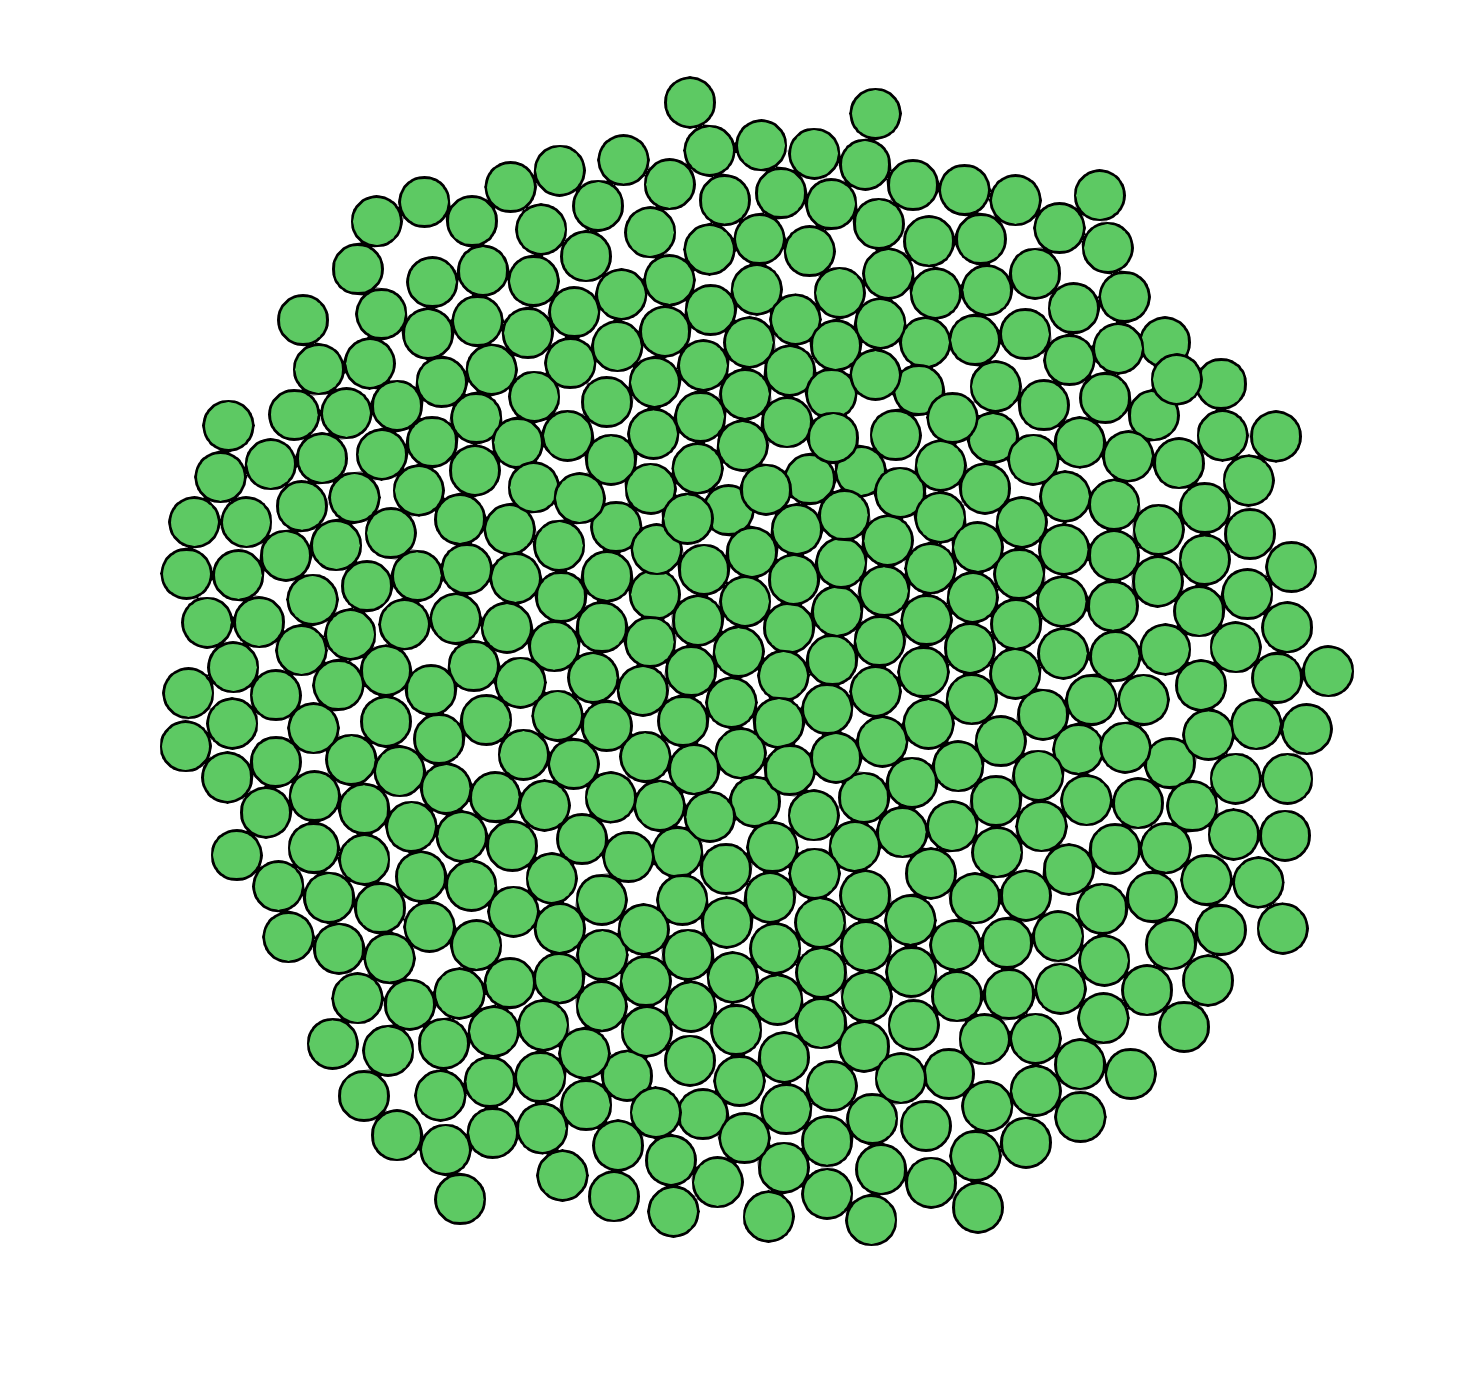
\includegraphics[width=\linewidth,trim=100 80 100 80,clip]{../movies/CyclingClock/image.0452.png}
      \caption{$t=10$ h}
    \end{subfigure}
    \hfill
    \begin{subfigure}[t]{0.19\textwidth}
      \centering
      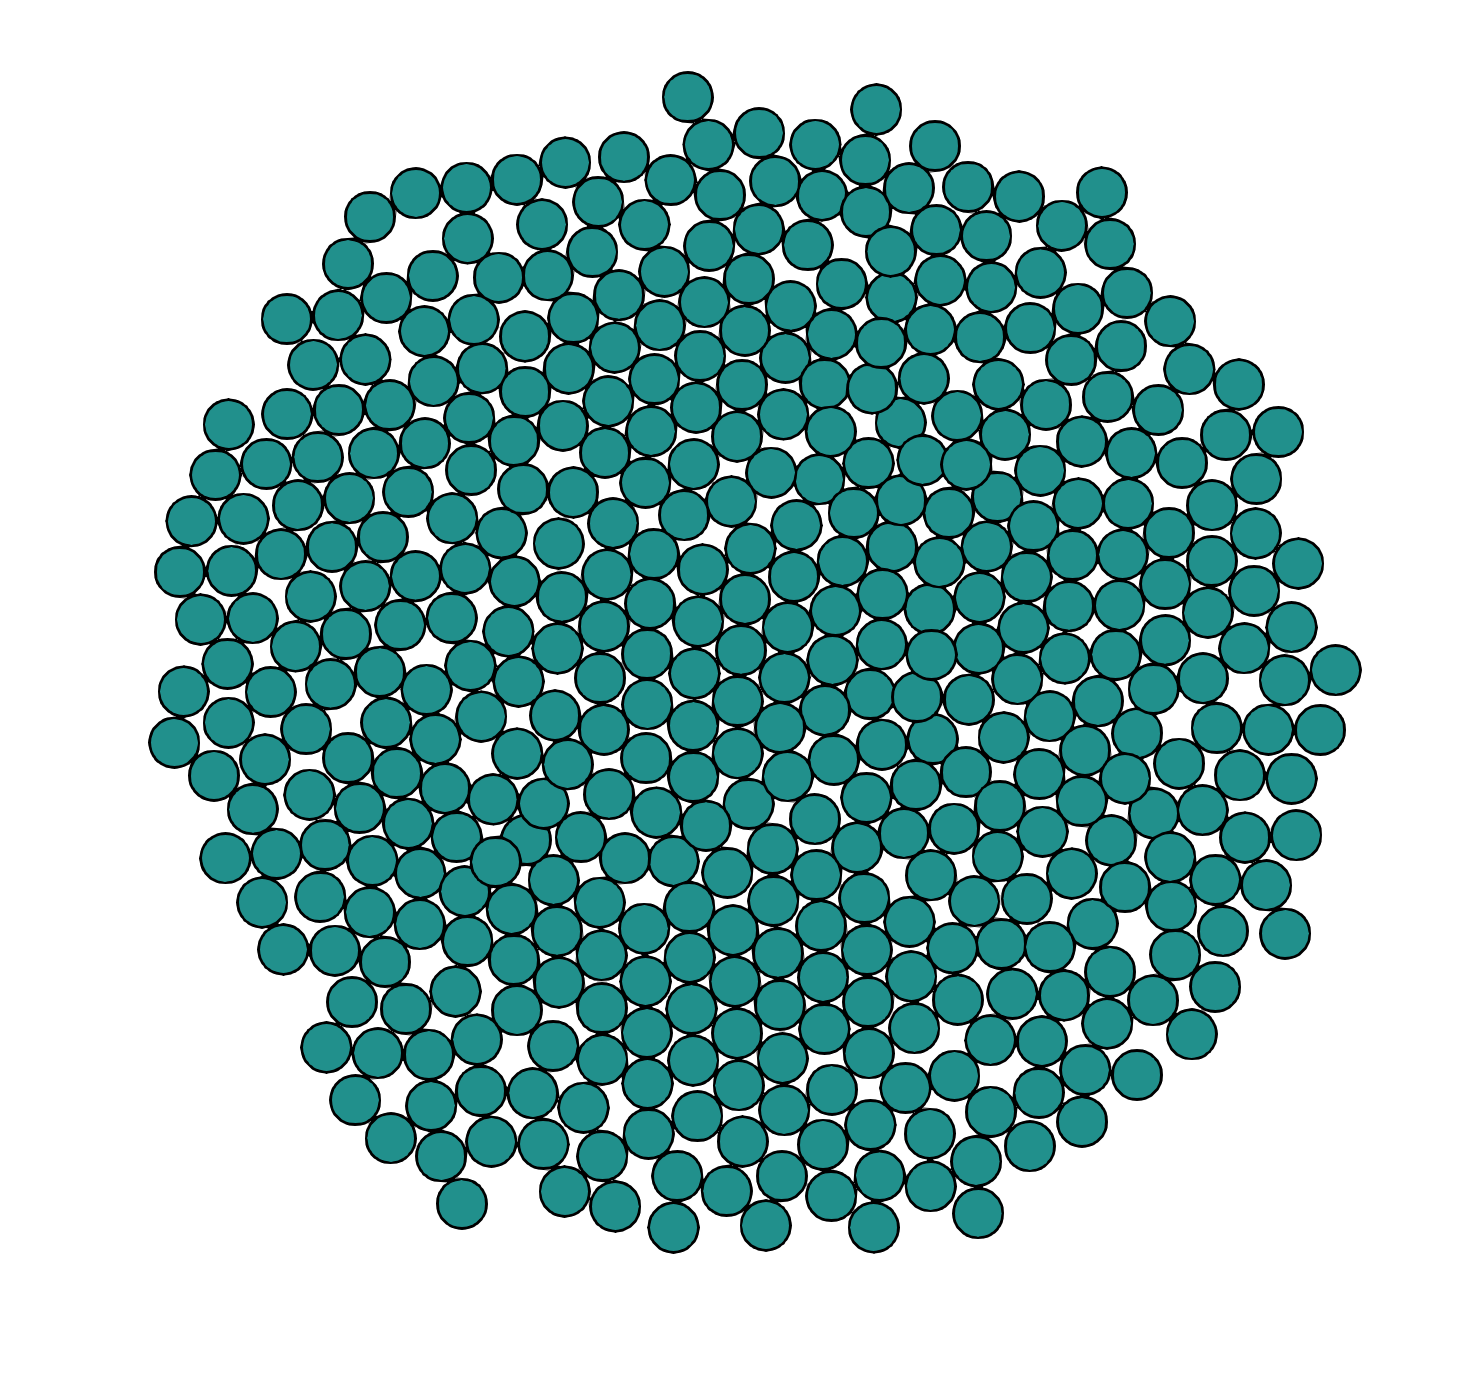
\includegraphics[width=\linewidth,trim=100 80 100 80,clip]{../movies/CyclingClock/image.0456.png}
      \caption{$t=12$ h}
    \end{subfigure}
    \hfill
    \begin{subfigure}[t]{0.19\textwidth}
      \centering
      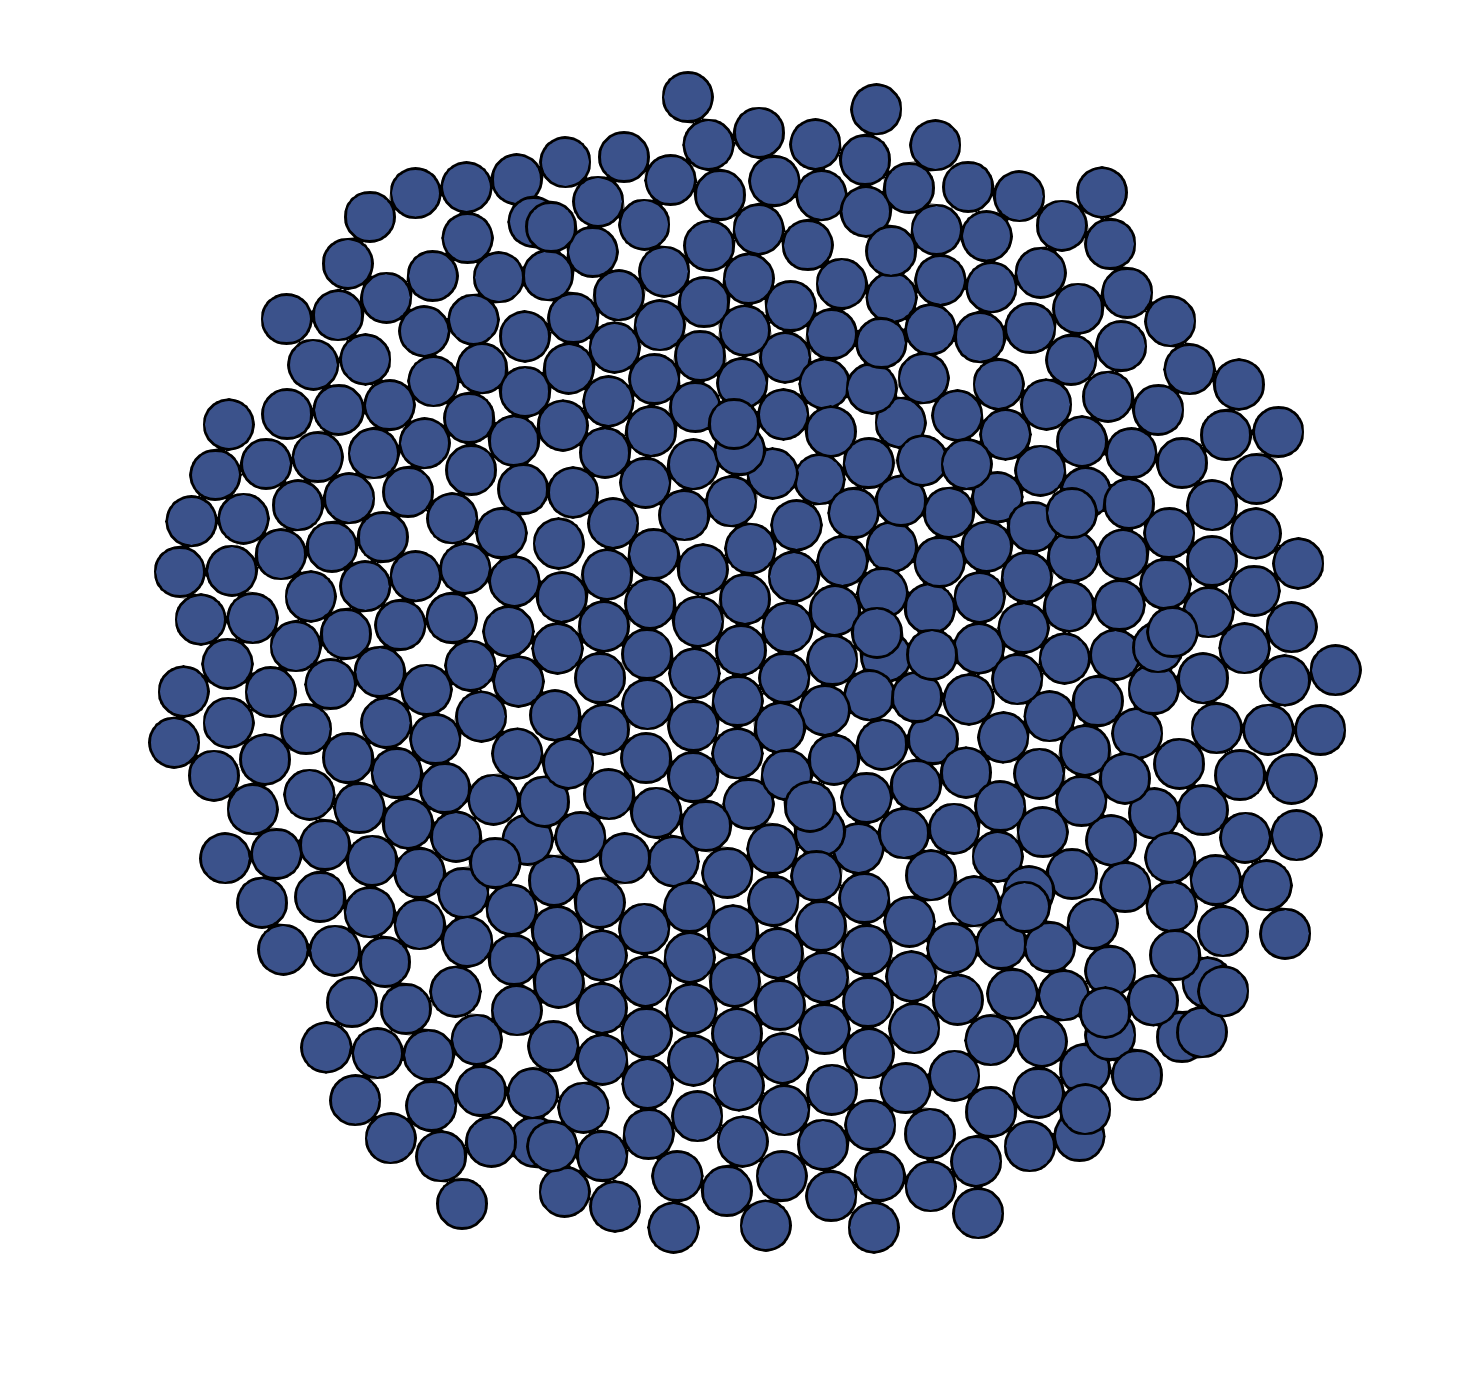
\includegraphics[width=\linewidth,trim=100 80 100 80,clip]{../movies/CyclingClock/image.0460.png}
      \caption{$t=14$ h}
    \end{subfigure}
    \hfill
    \begin{subfigure}[t]{0.19\textwidth}
      \centering
      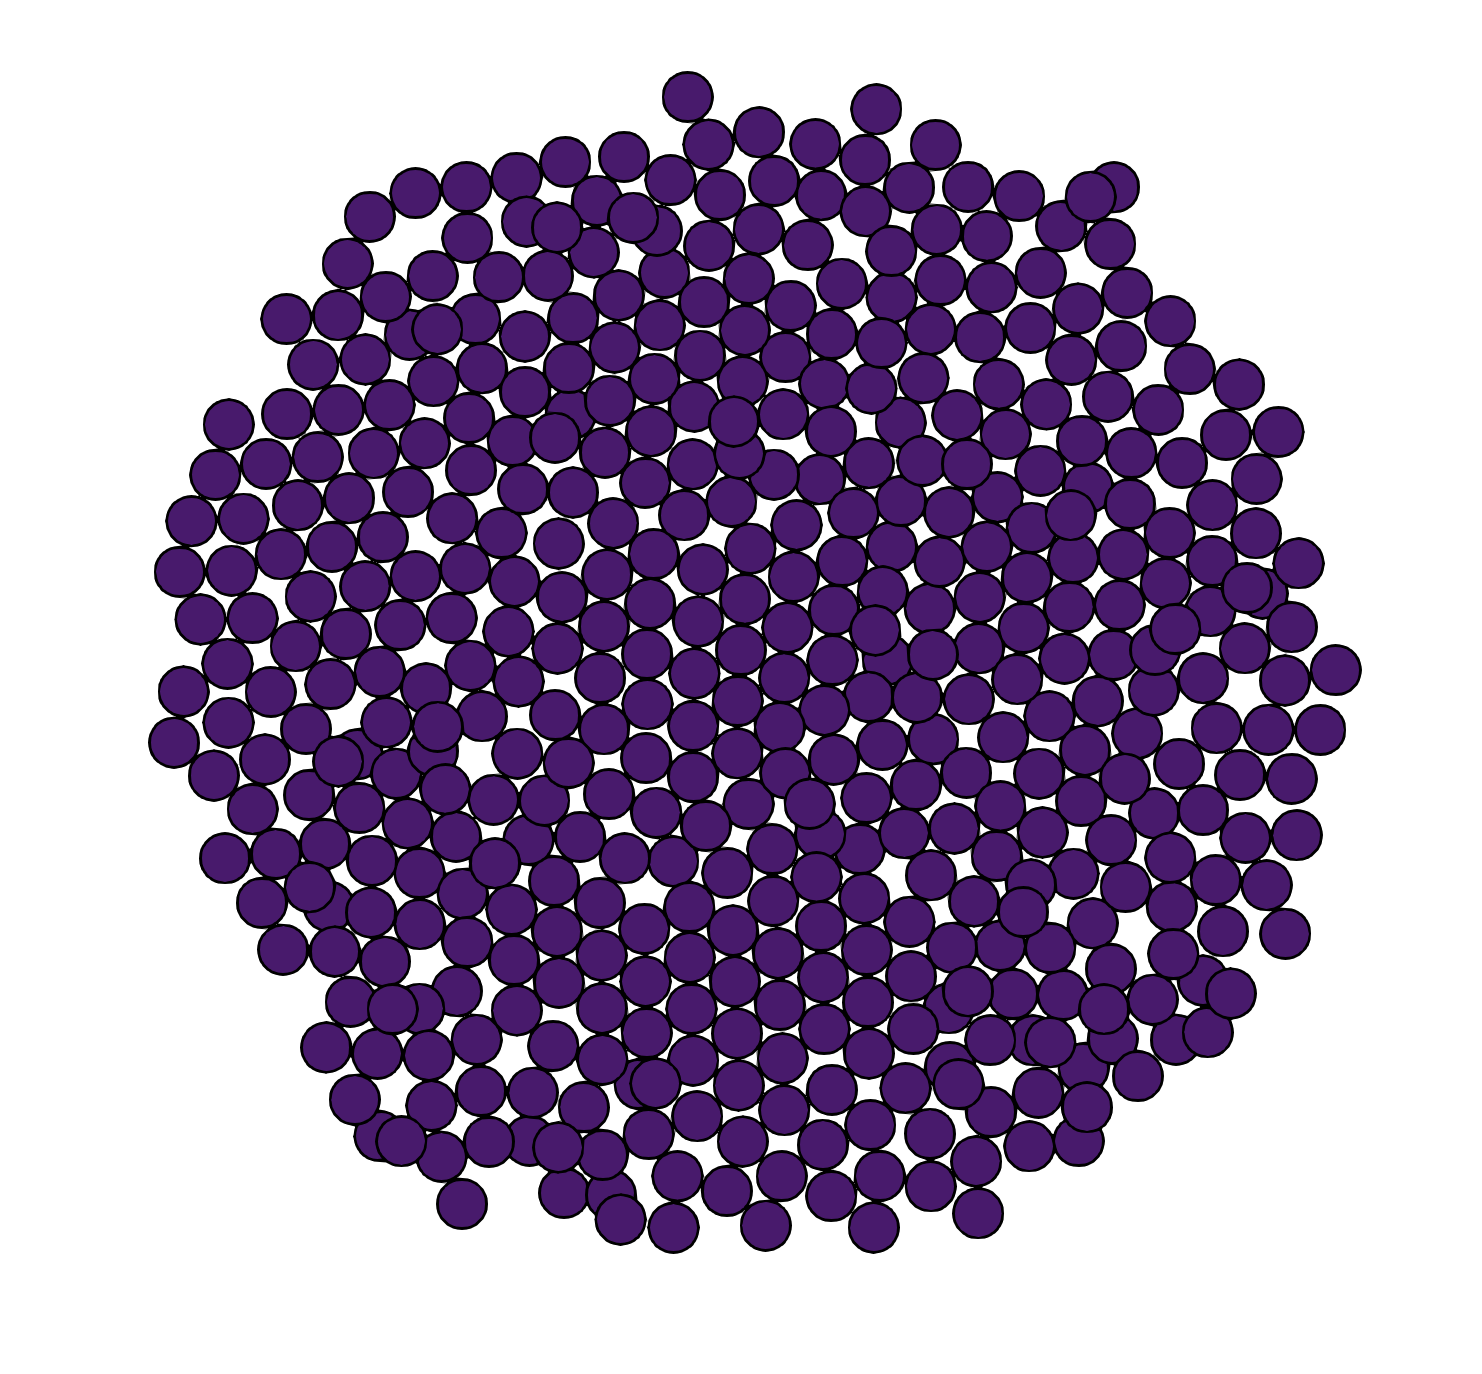
\includegraphics[width=\linewidth,trim=100 80 100 80,clip]{../movies/CyclingClock/image.0464.png}
      \caption{$t=16$ h}
    \end{subfigure}
    \hfill
    \begin{subfigure}[t]{0.19\textwidth}
      \centering
      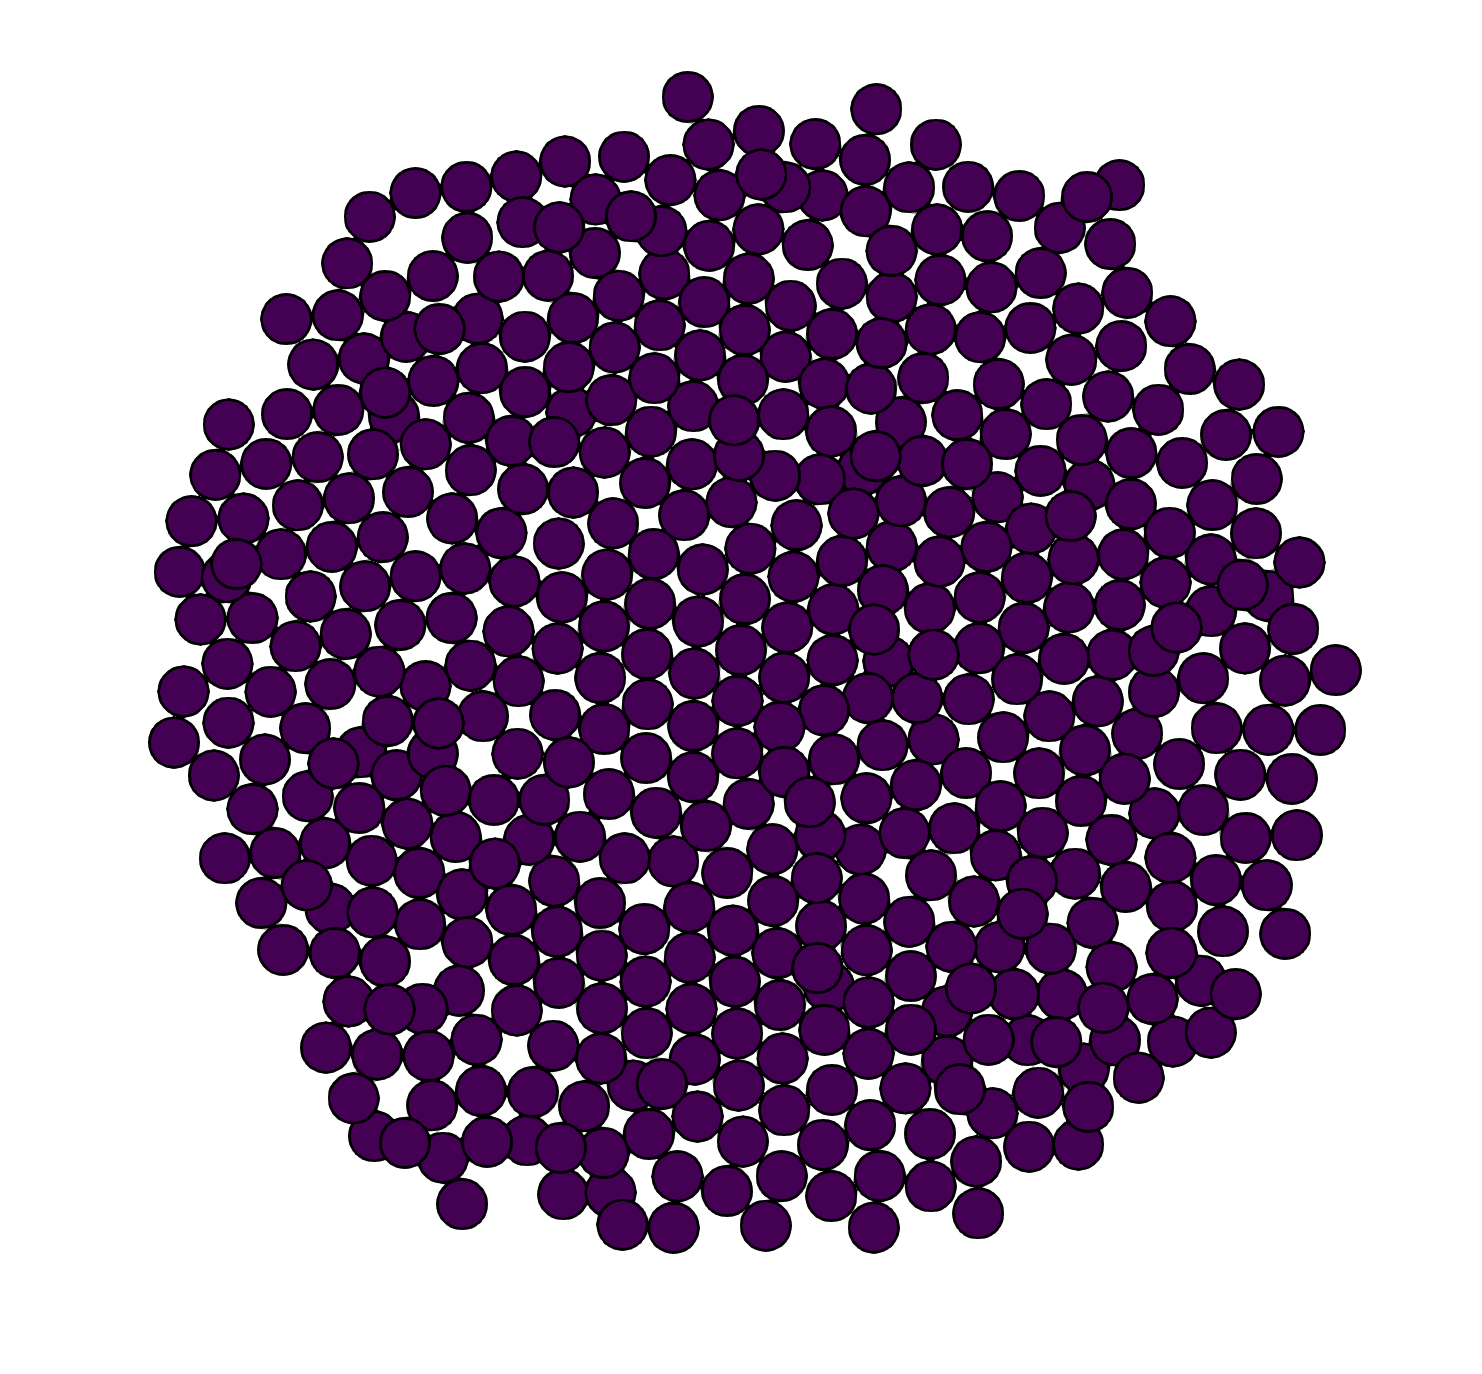
\includegraphics[width=\linewidth,trim=100 80 100 80,clip]{../movies/CyclingClock/image.0468.png}
      \caption{$t=18$ h}
    \end{subfigure}

    \medskip
    \begin{subfigure}[t]{0.19\textwidth}
      \centering
      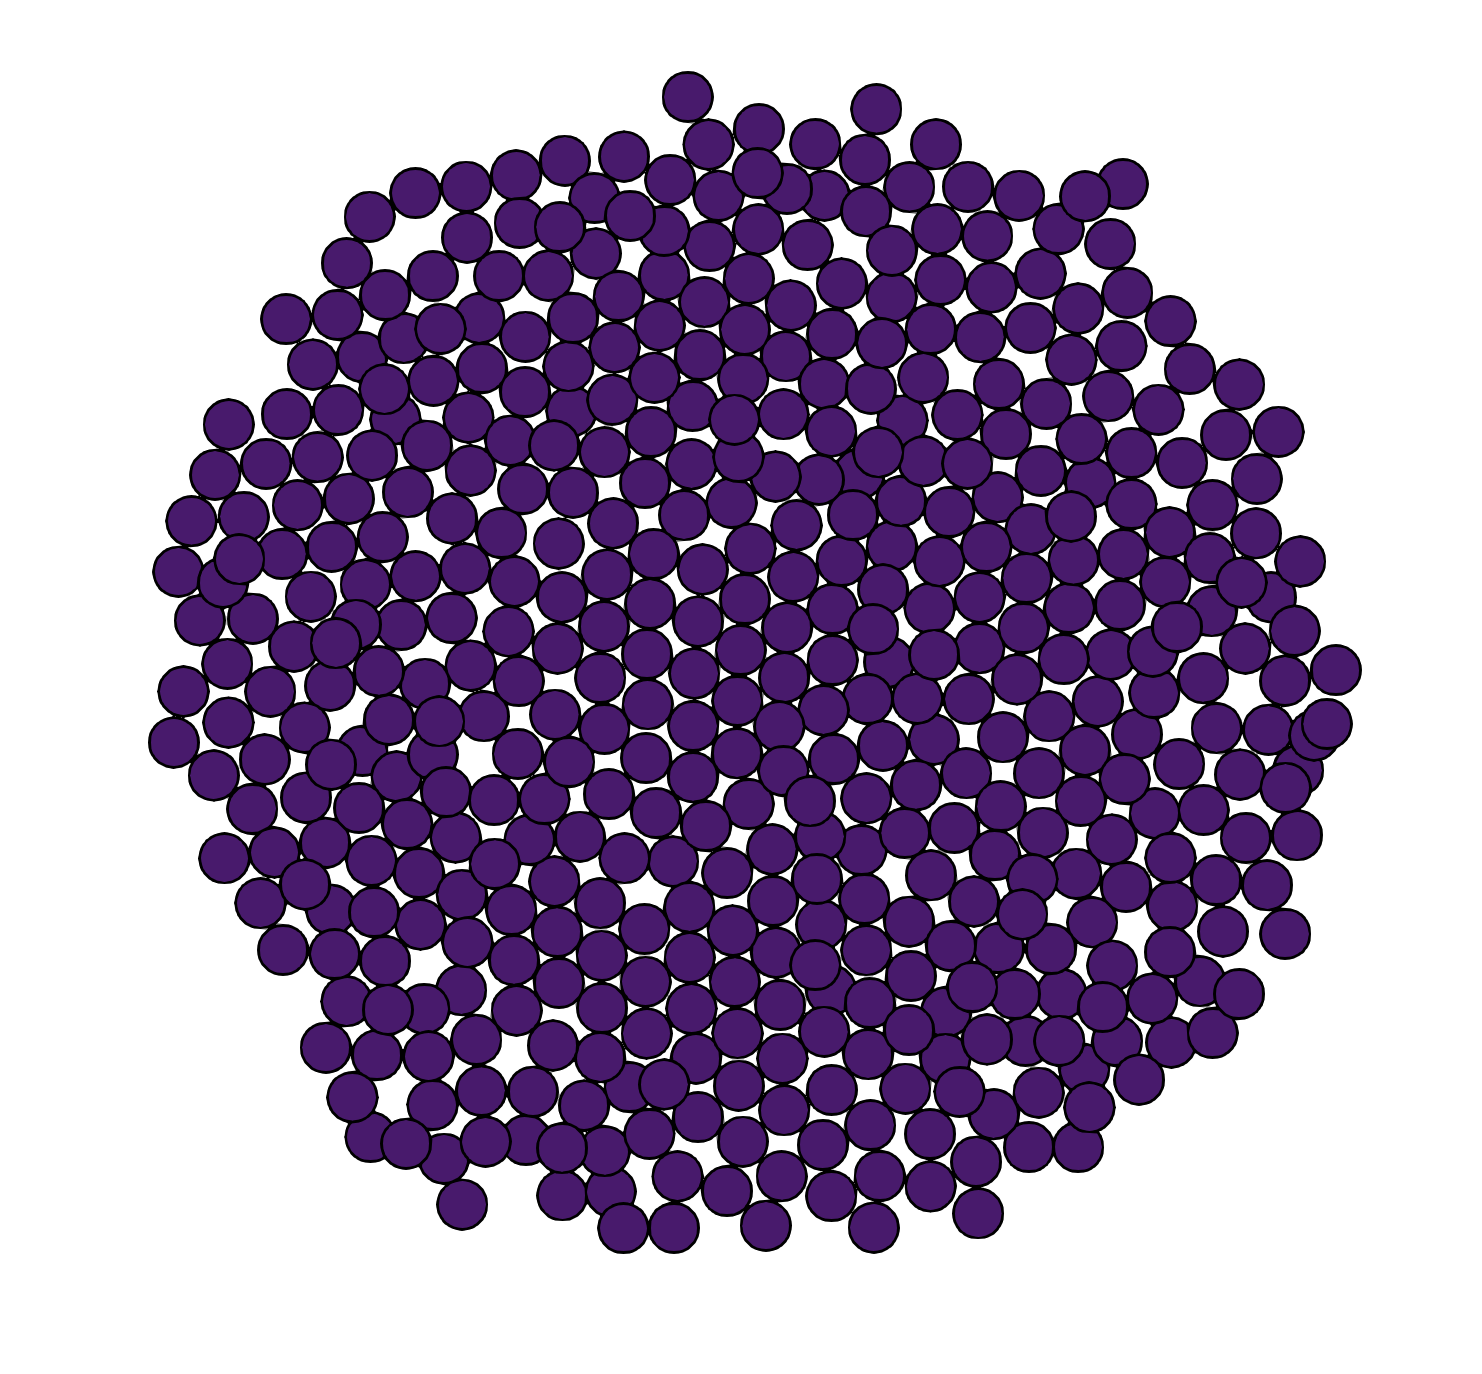
\includegraphics[width=\linewidth,trim=100 80 100 80,clip]{../movies/CyclingClock/image.0472.png}
      \caption{$t=20$ h}
    \end{subfigure}
    \hfill
    \begin{subfigure}[t]{0.19\textwidth}
      \centering
      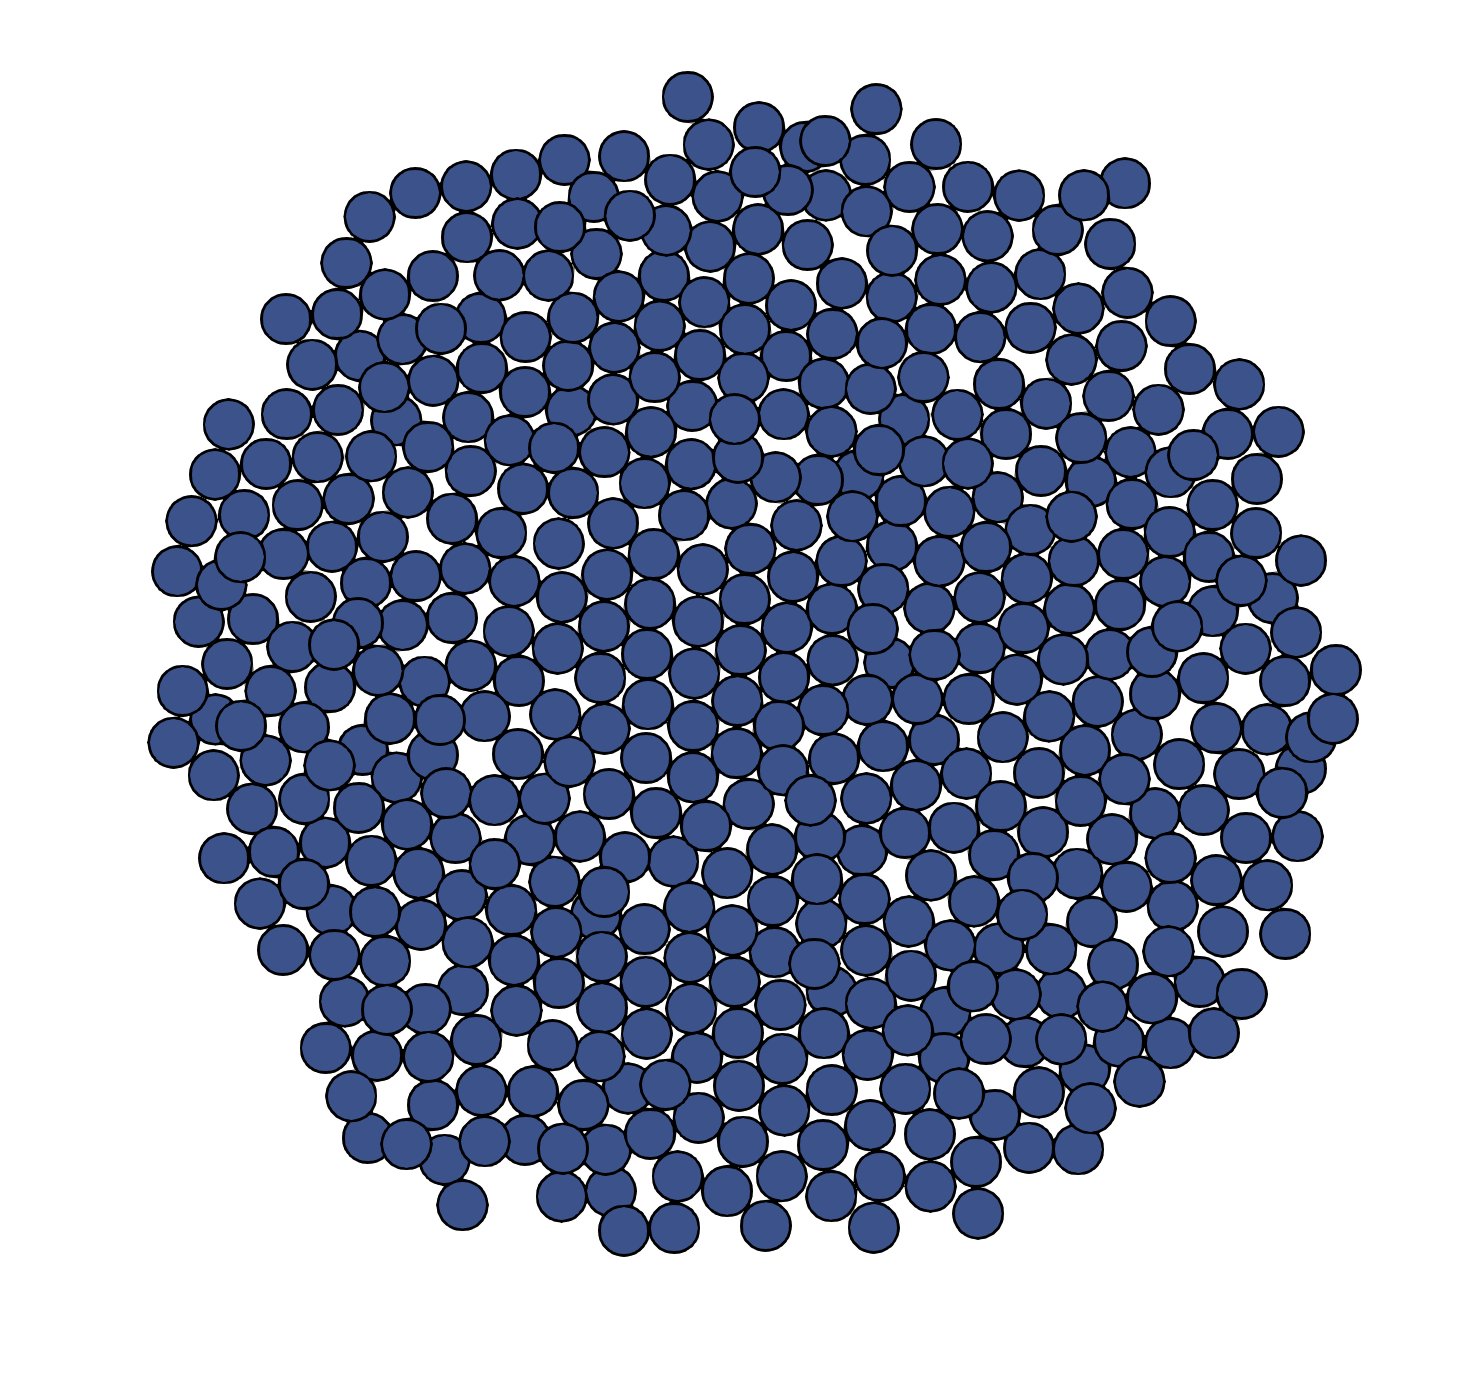
\includegraphics[width=\linewidth,trim=100 80 100 80,clip]{../movies/CyclingClock/image.0476.png}
      \caption{$t=22$ h}
    \end{subfigure}
    \hfill
    \begin{subfigure}[t]{0.19\textwidth}
      \centering
      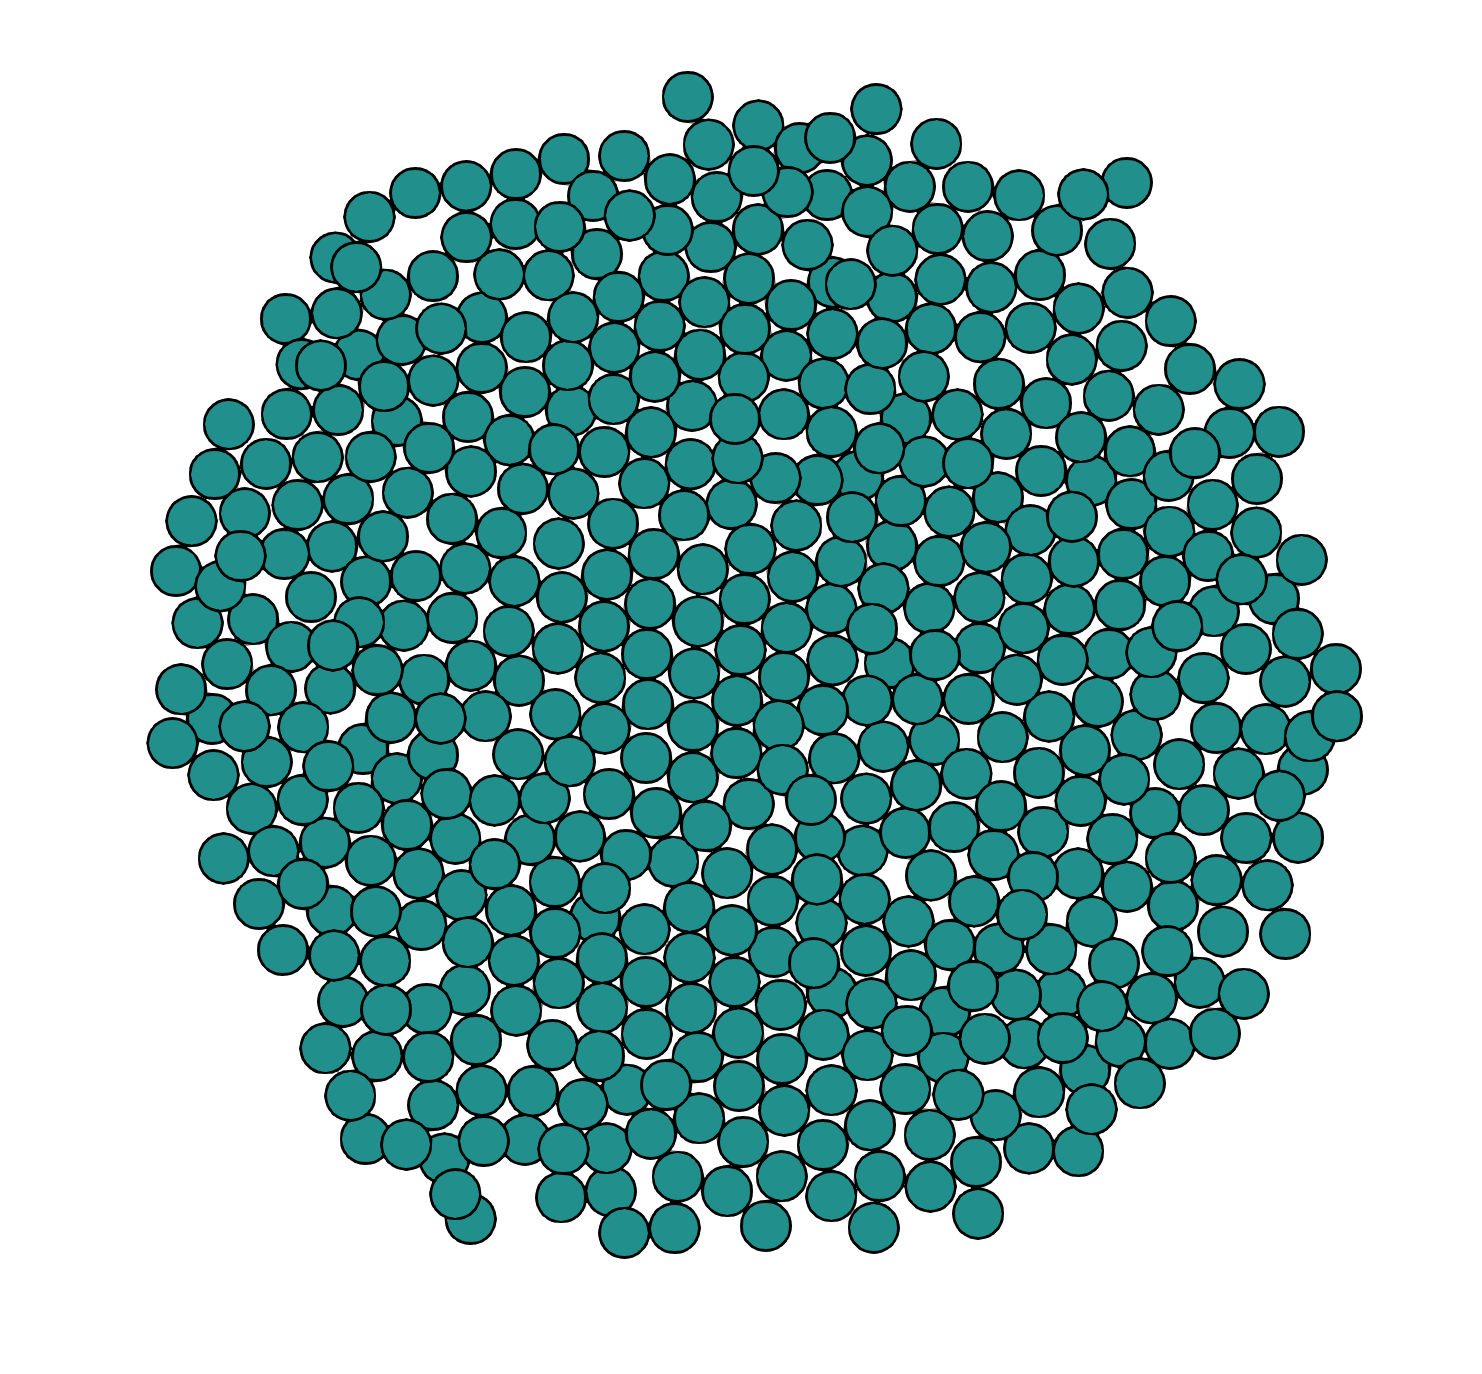
\includegraphics[width=\linewidth,trim=100 80 100 80,clip]{../movies/CyclingClock/image.0480.png}
      \caption{$t=24$ h}
    \end{subfigure}
  \end{minipage}%
  \hfill
  \begin{minipage}[c]{0.10\textwidth}
    \centering
    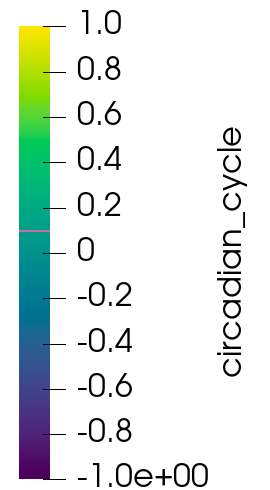
\includegraphics[width=\linewidth,trim=0 0 68 0,clip]{../movies/CyclingClock/legend.png}
  \end{minipage}
  \caption{All-cycling simulation snapshots over a 24-hour window at 2-hour intervals. Cell Color represents the position in the circadian cycle.}\label{fig:cycling-24h-2hourly}
\end{figure}

\bibliographystyle{plain}
\bibliography{TestClocksCompetition}

\end{document}
